% Options for packages loaded elsewhere
% Options for packages loaded elsewhere
\PassOptionsToPackage{unicode}{hyperref}
\PassOptionsToPackage{hyphens}{url}
\PassOptionsToPackage{dvipsnames,svgnames,x11names}{xcolor}
%
\documentclass[
  portuguese,
  11pt,
  a4paper,
  DIV=11,
  numbers=noendperiod]{scrreprt}
\usepackage{xcolor}
\usepackage[left=2.5cm,top=2.5cm,right=2.5cm,bottom=2.5cm]{geometry}
\usepackage{amsmath,amssymb}
\setcounter{secnumdepth}{5}
\usepackage{iftex}
\ifPDFTeX
  \usepackage[T1]{fontenc}
  \usepackage[utf8]{inputenc}
  \usepackage{textcomp} % provide euro and other symbols
\else % if luatex or xetex
  \usepackage{unicode-math} % this also loads fontspec
  \defaultfontfeatures{Scale=MatchLowercase}
  \defaultfontfeatures[\rmfamily]{Ligatures=TeX,Scale=1}
\fi
\usepackage{lmodern}
\ifPDFTeX\else
  % xetex/luatex font selection
\fi
% Use upquote if available, for straight quotes in verbatim environments
\IfFileExists{upquote.sty}{\usepackage{upquote}}{}
\IfFileExists{microtype.sty}{% use microtype if available
  \usepackage[]{microtype}
  \UseMicrotypeSet[protrusion]{basicmath} % disable protrusion for tt fonts
}{}
% Make \paragraph and \subparagraph free-standing
\makeatletter
\ifx\paragraph\undefined\else
  \let\oldparagraph\paragraph
  \renewcommand{\paragraph}{
    \@ifstar
      \xxxParagraphStar
      \xxxParagraphNoStar
  }
  \newcommand{\xxxParagraphStar}[1]{\oldparagraph*{#1}\mbox{}}
  \newcommand{\xxxParagraphNoStar}[1]{\oldparagraph{#1}\mbox{}}
\fi
\ifx\subparagraph\undefined\else
  \let\oldsubparagraph\subparagraph
  \renewcommand{\subparagraph}{
    \@ifstar
      \xxxSubParagraphStar
      \xxxSubParagraphNoStar
  }
  \newcommand{\xxxSubParagraphStar}[1]{\oldsubparagraph*{#1}\mbox{}}
  \newcommand{\xxxSubParagraphNoStar}[1]{\oldsubparagraph{#1}\mbox{}}
\fi
\makeatother


\usepackage{longtable,booktabs,array}
\usepackage{calc} % for calculating minipage widths
% Correct order of tables after \paragraph or \subparagraph
\usepackage{etoolbox}
\makeatletter
\patchcmd\longtable{\par}{\if@noskipsec\mbox{}\fi\par}{}{}
\makeatother
% Allow footnotes in longtable head/foot
\IfFileExists{footnotehyper.sty}{\usepackage{footnotehyper}}{\usepackage{footnote}}
\makesavenoteenv{longtable}
\usepackage{graphicx}
\makeatletter
\newsavebox\pandoc@box
\newcommand*\pandocbounded[1]{% scales image to fit in text height/width
  \sbox\pandoc@box{#1}%
  \Gscale@div\@tempa{\textheight}{\dimexpr\ht\pandoc@box+\dp\pandoc@box\relax}%
  \Gscale@div\@tempb{\linewidth}{\wd\pandoc@box}%
  \ifdim\@tempb\p@<\@tempa\p@\let\@tempa\@tempb\fi% select the smaller of both
  \ifdim\@tempa\p@<\p@\scalebox{\@tempa}{\usebox\pandoc@box}%
  \else\usebox{\pandoc@box}%
  \fi%
}
% Set default figure placement to htbp
\def\fps@figure{htbp}
\makeatother



\ifLuaTeX
\usepackage[bidi=basic]{babel}
\else
\usepackage[bidi=default]{babel}
\fi
% get rid of language-specific shorthands (see #6817):
\let\LanguageShortHands\languageshorthands
\def\languageshorthands#1{}


\setlength{\emergencystretch}{3em} % prevent overfull lines

\providecommand{\tightlist}{%
  \setlength{\itemsep}{0pt}\setlength{\parskip}{0pt}}



 


\usepackage{booktabs}
\usepackage{caption}
\usepackage{longtable}
\usepackage{colortbl}
\usepackage{array}
\usepackage{anyfontsize}
\usepackage{multirow}
\KOMAoption{captions}{tableheading}
\usepackage{indentfirst}
\usepackage{latexsym,amssymb,amsmath,amsfonts}
\usepackage{graphicx} % Figuras
\usepackage{latexsym, amssymb, amsmath, amsfonts, amsthm} % Formatação Matemática
\usepackage{xcolor}
\usepackage{float, caption}
\floatplacement{table}{H}
\floatplacement{figure}{H}
\captionsetup[table]{position=above}
\captionsetup[figure]{position=below}
\makeatletter
\@ifpackageloaded{bookmark}{}{\usepackage{bookmark}}
\makeatother
\makeatletter
\@ifpackageloaded{caption}{}{\usepackage{caption}}
\AtBeginDocument{%
\ifdefined\contentsname
  \renewcommand*\contentsname{Índice}
\else
  \newcommand\contentsname{Índice}
\fi
\ifdefined\listfigurename
  \renewcommand*\listfigurename{Lista de Figuras}
\else
  \newcommand\listfigurename{Lista de Figuras}
\fi
\ifdefined\listtablename
  \renewcommand*\listtablename{Lista de Tabelas}
\else
  \newcommand\listtablename{Lista de Tabelas}
\fi
\ifdefined\figurename
  \renewcommand*\figurename{Figura}
\else
  \newcommand\figurename{Figura}
\fi
\ifdefined\tablename
  \renewcommand*\tablename{Tabela}
\else
  \newcommand\tablename{Tabela}
\fi
}
\@ifpackageloaded{float}{}{\usepackage{float}}
\floatstyle{ruled}
\@ifundefined{c@chapter}{\newfloat{codelisting}{h}{lop}}{\newfloat{codelisting}{h}{lop}[chapter]}
\floatname{codelisting}{Listagem}
\newcommand*\listoflistings{\listof{codelisting}{Lista de Listagens}}
\makeatother
\makeatletter
\makeatother
\makeatletter
\@ifpackageloaded{caption}{}{\usepackage{caption}}
\@ifpackageloaded{subcaption}{}{\usepackage{subcaption}}
\makeatother
\usepackage{bookmark}
\IfFileExists{xurl.sty}{\usepackage{xurl}}{} % add URL line breaks if available
\urlstyle{same}
\hypersetup{
  pdftitle={TEORIA DE RESPOSTA AO ITEM},
  pdfauthor={Mário Diego Rocha Valente; Breno Cauã Rodrigues da Silva},
  pdflang={pt},
  colorlinks=true,
  linkcolor={blue},
  filecolor={Maroon},
  citecolor={Blue},
  urlcolor={Blue},
  pdfcreator={LaTeX via pandoc}}


\title{TEORIA DE RESPOSTA AO ITEM}
\usepackage{etoolbox}
\makeatletter
\providecommand{\subtitle}[1]{% add subtitle to \maketitle
  \apptocmd{\@title}{\par {\large #1 \par}}{}{}
}
\makeatother
\subtitle{COM DADOS DO ENADE}
\author{Mário Diego Rocha Valente \and Breno Cauã Rodrigues da Silva}
\date{}
\begin{document}
\maketitle

\renewcommand*\contentsname{Índice}
{
\hypersetup{linkcolor=}
\setcounter{tocdepth}{2}
\tableofcontents
}

\bookmarksetup{startatroot}

\chapter*{Prefácio}\label{prefuxe1cio}
\addcontentsline{toc}{chapter}{Prefácio}

\markboth{Prefácio}{Prefácio}

Na Edumetria\ldots{}

\begin{center}\rule{0.5\linewidth}{0.5pt}\end{center}

Este é um \textbf{Quarto Book}. Para saber mais sobre \textbf{Quarto
Book}, visite \url{https://quarto.org/docs/books/}.

\begin{center}\rule{0.5\linewidth}{0.5pt}\end{center}

\part{ANÁLISE DO ENADE POR CURSOS}

\bookmarksetup{startatroot}

\chapter{Curso de Bacharelado em Sistemas de
Informação}\label{curso-de-bacharelado-em-sistemas-de-informauxe7uxe3o}

\section{Introdução}\label{introduuxe7uxe3o}

\section{Análise Descritiva dos
Itens}\label{anuxe1lise-descritiva-dos-itens}

\section{Análise via Teoria Clássica dos Testes
(TCT)}\label{anuxe1lise-via-teoria-cluxe1ssica-dos-testes-tct}

\subsection{Tabela de Frequência (Absoluta e Relativa) das Alternativas
de
Respostas}\label{tabela-de-frequuxeancia-absoluta-e-relativa-das-alternativas-de-respostas}

Veja, a seguir, a Tabela~\ref{tbl-FREQ_ALTERNATIVE_ABS} e
Tabela~\ref{tbl-FREQ_ALTERNATIVE_REL}. Que mostram, respectivamente, a
distribuição de frequências absolutas alternativas às alternativas de
resposta.

\begin{table}

\caption{\label{tbl-FREQ_ALTERNATIVE_ABS}Frequências das Alternativas de
Respostas por Item.}

\centering{

\fontsize{12.0pt}{14.0pt}\selectfont
\begin{tabular*}{\linewidth}{@{\extracolsep{\fill}}cccccccccc}
\toprule
\textbf{Item} & \textbf{Gabarito} & \textbf{Branco} & \textbf{Mútiplas} & \textbf{A} & \textbf{B} & \textbf{C} & \textbf{D} & \textbf{E} & \textbf{Válidas} \\ 
\midrule\addlinespace[2.5pt]
1\textordfeminine FG & C & 51 & 9 & 1.170 & 4.536 & 2.714 & 3.911 & 1.400 & 13.731 \\ 
2\textordfeminine FG & C & 23 & 22 & 1.360 & 767 & 7.462 & 1.909 & 2.248 & 13.746 \\ 
3\textordfeminine FG & B & 99 & 20 & 2.640 & 4.832 & 2.591 & 2.325 & 1.284 & 13.672 \\ 
4\textordfeminine FG & B & 17 & 20 & 767 & 9.042 & 373 & 1.450 & 2.122 & 13.754 \\ 
5\textordfeminine FG & C & 16 & 11 & 164 & 1.335 & 8.180 & 1.005 & 3.080 & 13.764 \\ 
6\textordfeminine FG & E & 20 & 15 & 598 & 439 & 564 & 383 & 11.772 & 13.756 \\ 
7\textordfeminine FG & A & 24 & 10 & 4.828 & 3.345 & 1.507 & 2.339 & 1.738 & 13.757 \\ 
8\textordfeminine FG & D & 27 & 9 & 420 & 1.378 & 1.670 & 6.802 & 3.485 & 13.755 \\ 
1\textordfeminine CE & C & 15 & 14 & 1.727 & 1.933 & 1.420 & 2.759 & 5.923 & 13.762 \\ 
2\textordfeminine CE & E & 16 & 19 & 2.944 & 3.691 & 1.999 & 2.957 & 2.165 & 13.756 \\ 
3\textordfeminine CE & A & 19 & 33 & 3.316 & 1.476 & 2.885 & 3.392 & 2.670 & 13.739 \\ 
4\textordfeminine CE & C & 35 & 16 & 2.522 & 2.403 & 2.925 & 3.499 & 2.391 & 13.740 \\ 
5\textordfeminine CE & E & 25 & 8 & 1.955 & 1.887 & 1.823 & 4.498 & 3.595 & 13.758 \\ 
6\textordfeminine CE & ANULADA (E) & 12 & 8 & 4.643 & 2.005 & 1.928 & 3.725 & 1.470 & 13.771 \\ 
7\textordfeminine CE & A & 22 & 7 & 1.684 & 3.109 & 2.582 & 4.101 & 2.286 & 13.762 \\ 
8\textordfeminine CE & D & 11 & 6 & 2.772 & 1.902 & 3.556 & 3.194 & 2.350 & 13.774 \\ 
9\textordfeminine CE & B & 20 & 13 & 3.634 & 2.519 & 1.739 & 2.657 & 3.209 & 13.758 \\ 
10\textordfeminine CE & B & 25 & 6 & 3.396 & 4.071 & 1.916 & 2.272 & 2.105 & 13.760 \\ 
11\textordfeminine CE & B & 21 & 11 & 3.031 & 2.938 & 2.218 & 3.250 & 2.322 & 13.759 \\ 
12\textordfeminine CE & E & 22 & 13 & 2.646 & 2.214 & 2.533 & 3.825 & 2.538 & 13.756 \\ 
13\textordfeminine CE & B & 31 & 15 & 2.903 & 2.558 & 2.297 & 3.561 & 2.426 & 13.745 \\ 
14\textordfeminine CE & D & 29 & 20 & 3.108 & 2.284 & 2.991 & 2.139 & 3.220 & 13.742 \\ 
15\textordfeminine CE & D & 29 & 17 & 2.315 & 2.745 & 2.207 & 4.129 & 2.349 & 13.745 \\ 
16\textordfeminine CE & B & 32 & 11 & 2.599 & 1.905 & 2.978 & 2.747 & 3.519 & 13.748 \\ 
17\textordfeminine CE & B & 32 & 2 & 2.427 & 2.013 & 2.788 & 4.153 & 2.376 & 13.757 \\ 
18\textordfeminine CE & E & 32 & 7 & 2.505 & 3.014 & 2.637 & 2.356 & 3.240 & 13.752 \\ 
19\textordfeminine CE & A & 41 & 8 & 2.061 & 3.237 & 2.821 & 2.816 & 2.807 & 13.742 \\ 
20\textordfeminine CE & E & 43 & 10 & 3.010 & 2.562 & 2.742 & 2.538 & 2.886 & 13.738 \\ 
21\textordfeminine CE & A & 34 & 13 & 2.188 & 1.811 & 3.133 & 2.767 & 3.845 & 13.744 \\ 
22\textordfeminine CE & C & 50 & 10 & 2.232 & 2.472 & 2.602 & 2.442 & 3.983 & 13.731 \\ 
23\textordfeminine CE & B & 49 & 17 & 2.984 & 1.799 & 3.103 & 2.581 & 3.258 & 13.725 \\ 
24\textordfeminine CE & D & 50 & 9 & 3.635 & 3.095 & 2.172 & 2.830 & 2.000 & 13.732 \\ 
25\textordfeminine CE & C & 58 & 14 & 3.428 & 1.757 & 3.440 & 2.852 & 2.242 & 13.719 \\ 
26\textordfeminine CE & C & 54 & 12 & 2.323 & 3.771 & 2.459 & 3.099 & 2.073 & 13.725 \\ 
27\textordfeminine CE & C & 73 & 7 & 2.022 & 2.844 & 2.682 & 4.208 & 1.955 & 13.711 \\ 
\bottomrule
\end{tabular*}
\begin{minipage}{\linewidth}
FG: Formação Geral; CE: Componente Específico.\\
\end{minipage}

}

\end{table}%

\begin{table}

\caption{\label{tbl-FREQ_ALTERNATIVE_REL}Frequências das Alternativas de
Respostas por Item.}

\centering{

\fontsize{12.0pt}{14.0pt}\selectfont
\begin{tabular*}{\linewidth}{@{\extracolsep{\fill}}cccccccc}
\toprule
\textbf{Item Especificado} & \textbf{Gabarito} & \textbf{A (\%)} & \textbf{B (\%)} & \textbf{C (\%)} & \textbf{D (\%)} & \textbf{E (\%)} & \textbf{Total (\%)} \\ 
\midrule\addlinespace[2.5pt]
1\textordfeminine FG & C & 8,52 & 33,03 & 19,77 & 28,48 & 10,20 & 100,00 \\ 
2\textordfeminine FG & C & 9,89 & 5,58 & 54,28 & 13,89 & 16,35 & 100,00 \\ 
3\textordfeminine FG & B & 19,31 & 35,34 & 18,95 & 17,01 & 9,39 & 100,00 \\ 
4\textordfeminine FG & B & 5,58 & 65,74 & 2,71 & 10,54 & 15,43 & 100,00 \\ 
5\textordfeminine FG & C & 1,19 & 9,70 & 59,43 & 7,30 & 22,38 & 100,00 \\ 
6\textordfeminine FG & E & 4,35 & 3,19 & 4,10 & 2,78 & 85,58 & 100,00 \\ 
7\textordfeminine FG & A & 35,09 & 24,31 & 10,95 & 17,00 & 12,63 & 100,00 \\ 
8\textordfeminine FG & D & 3,05 & 10,02 & 12,14 & 49,45 & 25,34 & 100,00 \\ 
1\textordfeminine CE & C & 12,55 & 14,05 & 10,32 & 20,05 & 43,04 & 100,00 \\ 
2\textordfeminine CE & E & 21,40 & 26,83 & 14,53 & 21,50 & 15,74 & 100,00 \\ 
3\textordfeminine CE & A & 24,14 & 10,74 & 21,00 & 24,69 & 19,43 & 100,00 \\ 
4\textordfeminine CE & C & 18,36 & 17,49 & 21,29 & 25,47 & 17,40 & 100,00 \\ 
5\textordfeminine CE & E & 14,21 & 13,72 & 13,25 & 32,69 & 26,13 & 100,00 \\ 
6\textordfeminine CE & ANULADA (E) & 33,72 & 14,56 & 14,00 & 27,05 & 10,67 & 100,00 \\ 
7\textordfeminine CE & A & 12,24 & 22,59 & 18,76 & 29,80 & 16,61 & 100,00 \\ 
8\textordfeminine CE & D & 20,12 & 13,81 & 25,82 & 23,19 & 17,06 & 100,00 \\ 
9\textordfeminine CE & B & 26,41 & 18,31 & 12,64 & 19,31 & 23,32 & 100,00 \\ 
10\textordfeminine CE & B & 24,68 & 29,59 & 13,92 & 16,51 & 15,30 & 100,00 \\ 
11\textordfeminine CE & B & 22,03 & 21,35 & 16,12 & 23,62 & 16,88 & 100,00 \\ 
12\textordfeminine CE & E & 19,24 & 16,09 & 18,41 & 27,81 & 18,45 & 100,00 \\ 
13\textordfeminine CE & B & 21,12 & 18,61 & 16,71 & 25,91 & 17,65 & 100,00 \\ 
14\textordfeminine CE & D & 22,62 & 16,62 & 21,77 & 15,57 & 23,43 & 100,00 \\ 
15\textordfeminine CE & D & 16,84 & 19,97 & 16,06 & 30,04 & 17,09 & 100,00 \\ 
16\textordfeminine CE & B & 18,90 & 13,86 & 21,66 & 19,98 & 25,60 & 100,00 \\ 
17\textordfeminine CE & B & 17,64 & 14,63 & 20,27 & 30,19 & 17,27 & 100,00 \\ 
18\textordfeminine CE & E & 18,22 & 21,92 & 19,18 & 17,13 & 23,56 & 100,00 \\ 
19\textordfeminine CE & A & 15,00 & 23,56 & 20,53 & 20,49 & 20,43 & 100,00 \\ 
20\textordfeminine CE & E & 21,91 & 18,65 & 19,96 & 18,47 & 21,01 & 100,00 \\ 
21\textordfeminine CE & A & 15,92 & 13,18 & 22,80 & 20,13 & 27,98 & 100,00 \\ 
22\textordfeminine CE & C & 16,26 & 18,00 & 18,95 & 17,78 & 29,01 & 100,00 \\ 
23\textordfeminine CE & B & 21,74 & 13,11 & 22,61 & 18,81 & 23,74 & 100,00 \\ 
24\textordfeminine CE & D & 26,47 & 22,54 & 15,82 & 20,61 & 14,56 & 100,00 \\ 
25\textordfeminine CE & C & 24,99 & 12,81 & 25,07 & 20,79 & 16,34 & 100,00 \\ 
26\textordfeminine CE & C & 16,93 & 27,48 & 17,92 & 22,58 & 15,10 & 100,00 \\ 
27\textordfeminine CE & C & 14,75 & 20,74 & 19,56 & 30,69 & 14,26 & 100,00 \\ 
\bottomrule
\end{tabular*}
\begin{minipage}{\linewidth}
FG: Formação Geral; CE: Componente Específico.\\
\end{minipage}

}

\end{table}%

\subsection{Tabela de Proporção de Acertos
(\%)}\label{tabela-de-proporuxe7uxe3o-de-acertos}

Veja, a seguir, a Tabela~\ref{tbl-PROP_HITS}. Que apresenta as
proporções de acertos para cada item.

\begin{table}

\caption{\label{tbl-PROP_HITS}Proporção de Acertos dos Itens.}

\centering{

\fontsize{12.0pt}{14.0pt}\selectfont
\begin{tabular*}{\linewidth}{@{\extracolsep{\fill}}ccc}
\toprule
\textbf{Item} & \textbf{Gabarito} & \textbf{Proporção de Acertos (\%)} \\ 
\midrule\addlinespace[2.5pt]
1\textordfeminine FG & C & 19,77 \\ 
2\textordfeminine FG & C & 54,28 \\ 
3\textordfeminine FG & B & 35,34 \\ 
4\textordfeminine FG & B & 65,74 \\ 
5\textordfeminine FG & C & 59,43 \\ 
6\textordfeminine FG & E & 85,58 \\ 
7\textordfeminine FG & A & 35,09 \\ 
8\textordfeminine FG & D & 49,45 \\ 
1\textordfeminine CE & C & 10,32 \\ 
2\textordfeminine CE & E & 15,74 \\ 
3\textordfeminine CE & A & 24,14 \\ 
4\textordfeminine CE & C & 21,29 \\ 
5\textordfeminine CE & E & 26,13 \\ 
6\textordfeminine CE & ANULADA (E) & NA \\ 
7\textordfeminine CE & A & 12,24 \\ 
8\textordfeminine CE & D & 23,19 \\ 
9\textordfeminine CE & B & 18,31 \\ 
10\textordfeminine CE & B & 29,59 \\ 
11\textordfeminine CE & B & 21,35 \\ 
12\textordfeminine CE & E & 18,45 \\ 
13\textordfeminine CE & B & 18,61 \\ 
14\textordfeminine CE & D & 15,57 \\ 
15\textordfeminine CE & D & 30,04 \\ 
16\textordfeminine CE & B & 13,86 \\ 
17\textordfeminine CE & B & 14,63 \\ 
18\textordfeminine CE & E & 23,56 \\ 
19\textordfeminine CE & A & 15,00 \\ 
20\textordfeminine CE & E & 21,01 \\ 
21\textordfeminine CE & A & 15,92 \\ 
22\textordfeminine CE & C & 18,95 \\ 
23\textordfeminine CE & B & 13,11 \\ 
24\textordfeminine CE & D & 20,61 \\ 
25\textordfeminine CE & C & 25,07 \\ 
26\textordfeminine CE & C & 17,92 \\ 
27\textordfeminine CE & C & 19,56 \\ 
\bottomrule
\end{tabular*}
\begin{minipage}{\linewidth}
FG: Formação Geral; CE: Componente Específico.\\
\end{minipage}

}

\end{table}%

\subsection{Histograma do Escore em Formação Geral, Componentes
Específicos e
Total}\label{histograma-do-escore-em-formauxe7uxe3o-geral-componentes-especuxedficos-e-total}

\begin{figure}[H]

\centering{

\pandocbounded{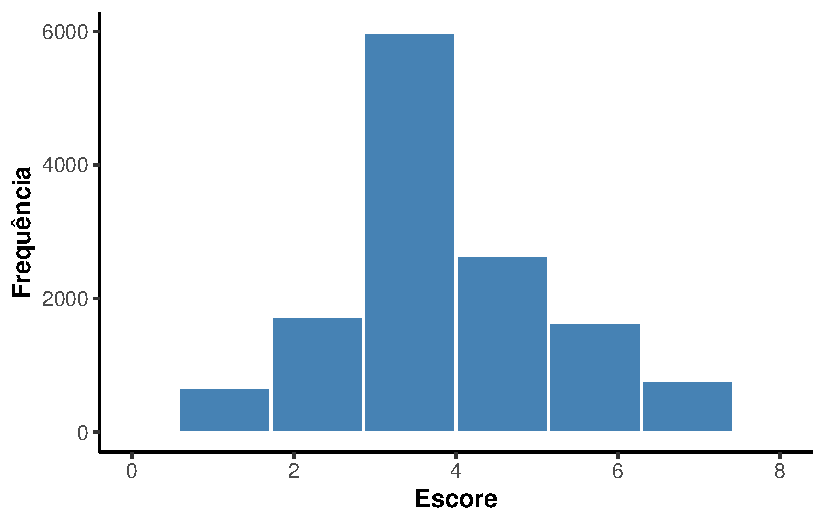
\includegraphics[keepaspectratio]{ANALYSIS_BY_COURSE/SISTEMAS_INFO_files/figure-pdf/fig-HIST_SCORE_FG-1.pdf}}

}

\caption{\label{fig-HIST_SCORE_FG}Histograma dos Escore dos
Participantes em Formação Geral.}

\end{figure}%

\begin{figure}[H]

\centering{

\pandocbounded{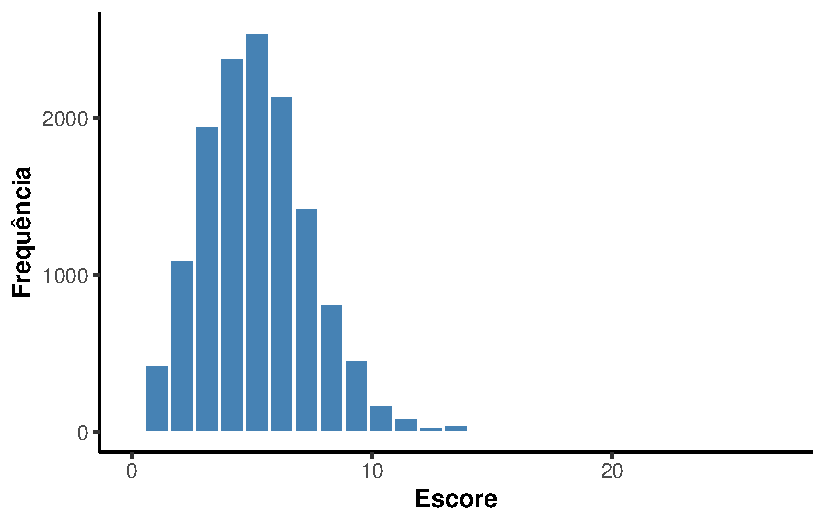
\includegraphics[keepaspectratio]{ANALYSIS_BY_COURSE/SISTEMAS_INFO_files/figure-pdf/fig-HIST_SCORE_CE-1.pdf}}

}

\caption{\label{fig-HIST_SCORE_CE}Histograma dos Escore dos
Participantes em Componentes Específicos.}

\end{figure}%

\begin{figure}[H]

\centering{

\pandocbounded{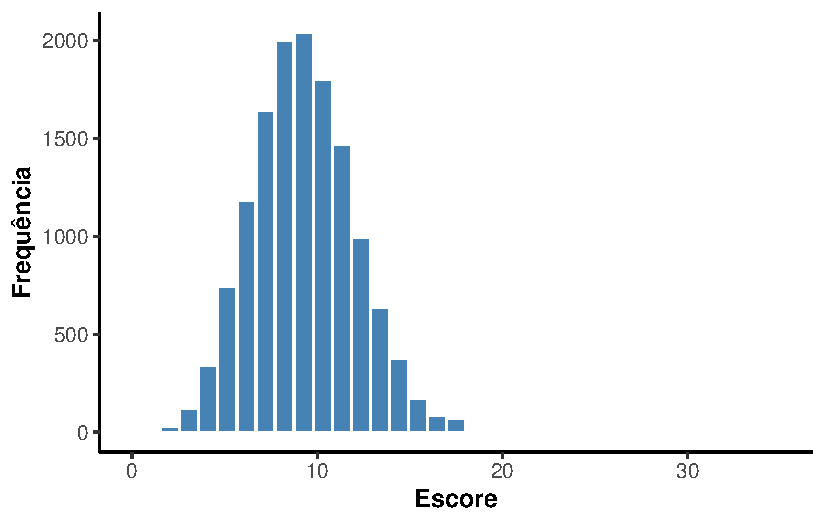
\includegraphics[keepaspectratio]{ANALYSIS_BY_COURSE/SISTEMAS_INFO_files/figure-pdf/fig-HIST_SCORE_TOTAL-1.pdf}}

}

\caption{\label{fig-HIST_SCORE_TOTAL}Histograma dos Escore Total dos
Participantes.}

\end{figure}%

\subsection{\texorpdfstring{Proporção de Acertos \emph{versus} Escore
por
Item}{Proporção de Acertos versus Escore por Item}}\label{proporuxe7uxe3o-de-acertos-versus-escore-por-item}

O objetivo desta análise é avaliar a \emph{Proporção de Acertos} por
\emph{Escore} de cada item.

A Figura~\ref{fig-PROP_HITS_AND_SCORE_BY_ITEM_1_A_5} apresenta a
proporção de acertos por escore para os itens de 1 (1º FG) a 5 (5º FG).

\begin{figure}[H]

\centering{

\pandocbounded{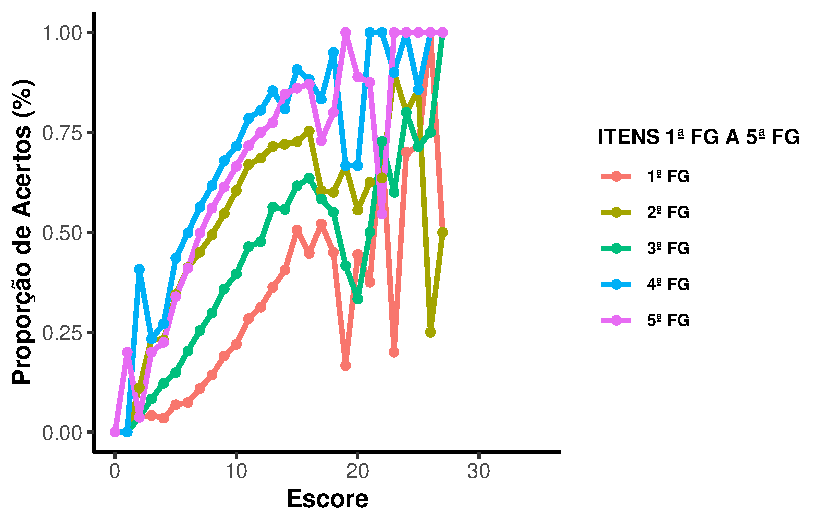
\includegraphics[keepaspectratio]{ANALYSIS_BY_COURSE/SISTEMAS_INFO_files/figure-pdf/fig-PROP_HITS_AND_SCORE_BY_ITEM_1_A_5-1.pdf}}

}

\caption{\label{fig-PROP_HITS_AND_SCORE_BY_ITEM_1_A_5}Proporção de
Acertos por Escore dos Itens de 1 (1º FG) a 5 (5º FG) da Prova do ENADE
para o Curso de Sitemas de Informação.}

\end{figure}%

A Figura~\ref{fig-PROP_HITS_AND_SCORE_BY_ITEM_6_A_10} apresenta a
proporção de acertos por escore para os itens de 6 (6º FG) a 10 (2º CE).

\begin{figure}[H]

\centering{

\pandocbounded{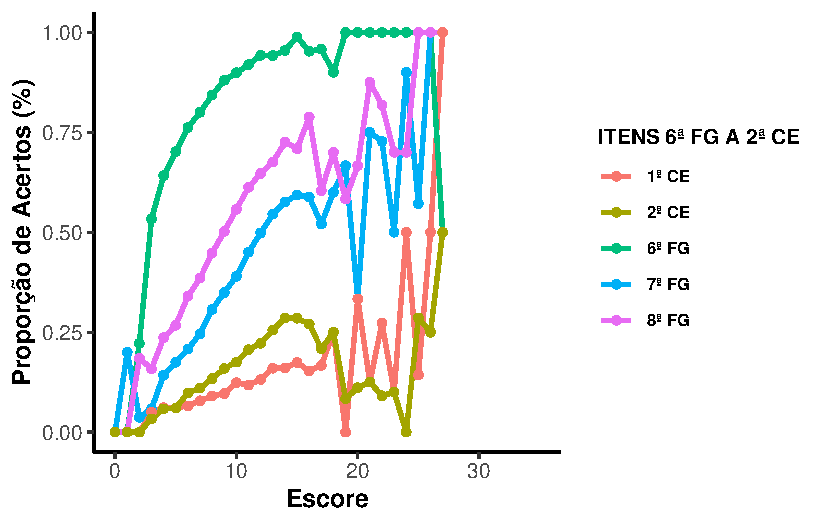
\includegraphics[keepaspectratio]{ANALYSIS_BY_COURSE/SISTEMAS_INFO_files/figure-pdf/fig-PROP_HITS_AND_SCORE_BY_ITEM_6_A_10-1.pdf}}

}

\caption{\label{fig-PROP_HITS_AND_SCORE_BY_ITEM_6_A_10}Proporção de
Acertos por Escore dos Itens de 6 (6º FG) a 10 (2º CE) da Prova do ENADE
para o Curso de Sitemas de Informação.}

\end{figure}%

A Figura~\ref{fig-PROP_HITS_AND_SCORE_BY_ITEM_11_A_15} apresenta a
proporção de acertos por escore para os itens de 11 (3º CE) a 15 (7º
CE).

\begin{figure}[H]

\centering{

\pandocbounded{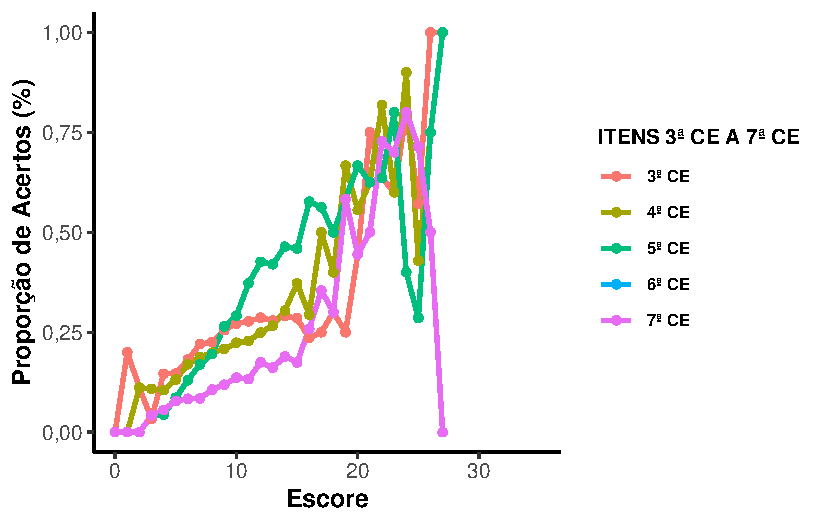
\includegraphics[keepaspectratio]{ANALYSIS_BY_COURSE/SISTEMAS_INFO_files/figure-pdf/fig-PROP_HITS_AND_SCORE_BY_ITEM_11_A_15-1.pdf}}

}

\caption{\label{fig-PROP_HITS_AND_SCORE_BY_ITEM_11_A_15}Proporção de
Acertos por Escore dos Itens de 11 (3º CE) a 15 (7º CE) da Prova do
ENADE para o Curso de Sitemas de Informação.}

\end{figure}%

A Figura~\ref{fig-PROP_HITS_AND_SCORE_BY_ITEM_16_A_20} apresenta a
proporção de acertos por escore para os itens de 16 (8º CE) a 20 (12º
CE).

\begin{figure}[H]

\centering{

\pandocbounded{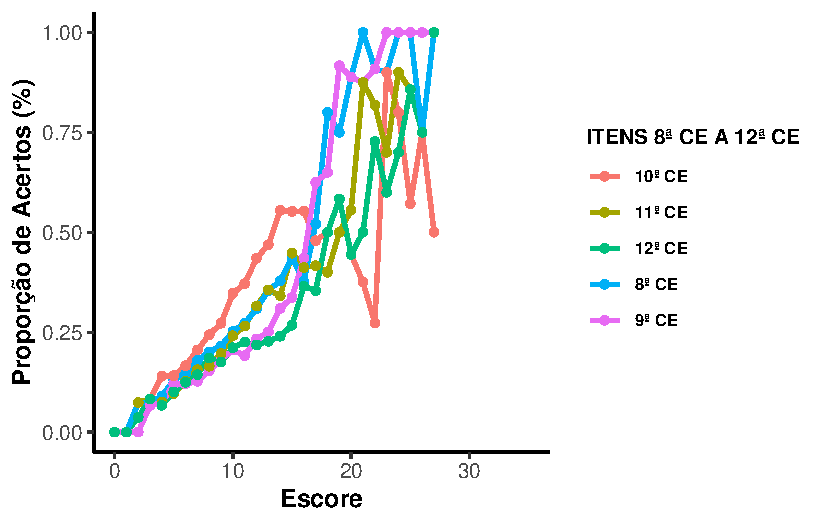
\includegraphics[keepaspectratio]{ANALYSIS_BY_COURSE/SISTEMAS_INFO_files/figure-pdf/fig-PROP_HITS_AND_SCORE_BY_ITEM_16_A_20-1.pdf}}

}

\caption{\label{fig-PROP_HITS_AND_SCORE_BY_ITEM_16_A_20}Proporção de
Acertos por Escore dos Itens de 16 (8º CE) a 20 (12º CE) da Prova do
ENADE para o Curso de Sitemas de Informação.}

\end{figure}%

A Figura~\ref{fig-PROP_HITS_AND_SCORE_BY_ITEM_21_A_25} apresenta a
proporção de acertos por escore para os itens de 21 (13º CE) a 25 (17º
CE).

\begin{figure}[H]

\centering{

\pandocbounded{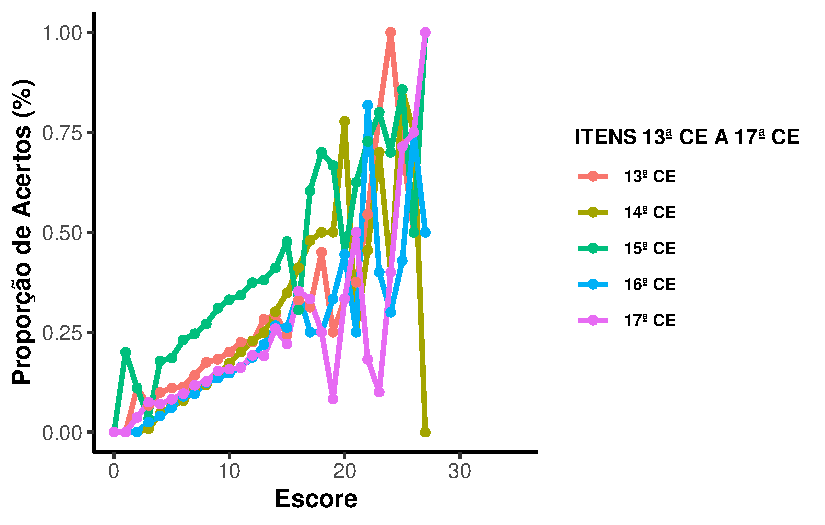
\includegraphics[keepaspectratio]{ANALYSIS_BY_COURSE/SISTEMAS_INFO_files/figure-pdf/fig-PROP_HITS_AND_SCORE_BY_ITEM_21_A_25-1.pdf}}

}

\caption{\label{fig-PROP_HITS_AND_SCORE_BY_ITEM_21_A_25}Proporção de
Acertos por Escore dos Itens de 21 (13º CE) a 25 (17º CE) da Prova do
ENADE para o Curso de Sitemas de Informação.}

\end{figure}%

A Figura~\ref{fig-PROP_HITS_AND_SCORE_BY_ITEM_26_A_30} apresenta a
proporção de acertos por escore para os itens de 26 (18º CE) a 30 (22º
CE).

\begin{figure}[H]

\centering{

\pandocbounded{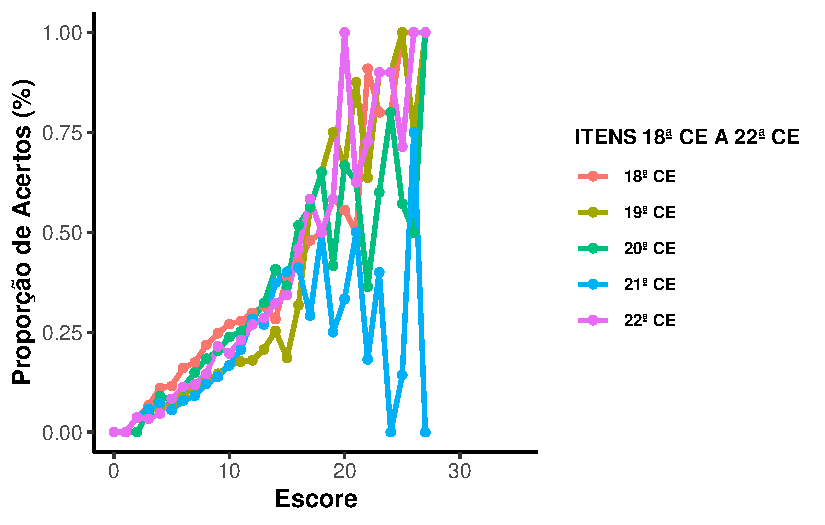
\includegraphics[keepaspectratio]{ANALYSIS_BY_COURSE/SISTEMAS_INFO_files/figure-pdf/fig-PROP_HITS_AND_SCORE_BY_ITEM_26_A_30-1.pdf}}

}

\caption{\label{fig-PROP_HITS_AND_SCORE_BY_ITEM_26_A_30}Proporção de
Acertos por Escore dos Itens de 26 (18º CE) a 30 (22º CE) da Prova do
ENADE para o Curso de Sitemas de Informação.}

\end{figure}%

A Figura~\ref{fig-PROP_HITS_AND_SCORE_BY_ITEM_31_A_35} apresenta a
proporção de acertos por escore para os itens de 31 (23º CE) a 35 (27º
CE).

\begin{figure}[H]

\centering{

\pandocbounded{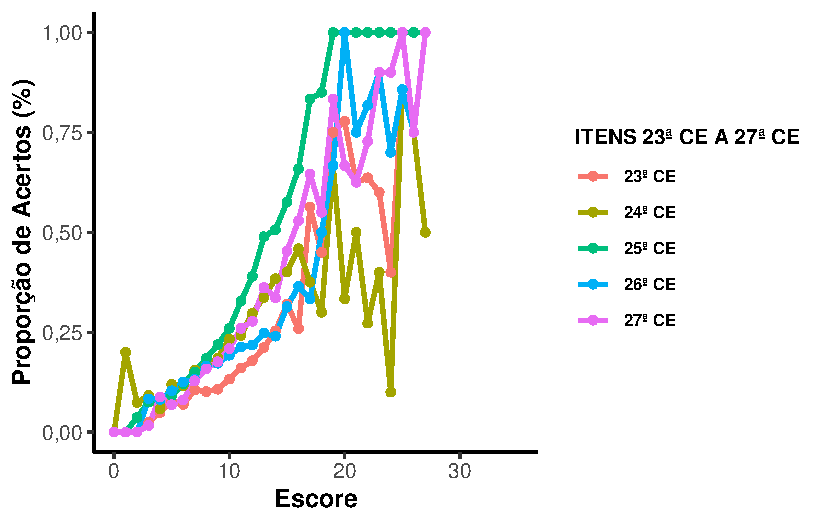
\includegraphics[keepaspectratio]{ANALYSIS_BY_COURSE/SISTEMAS_INFO_files/figure-pdf/fig-PROP_HITS_AND_SCORE_BY_ITEM_31_A_35-1.pdf}}

}

\caption{\label{fig-PROP_HITS_AND_SCORE_BY_ITEM_31_A_35}Proporção de
Acertos por Escore dos Itens de 31 (23º CE) a 35 (27º CE) da Prova do
ENADE para o Curso de Sitemas de Informação.}

\end{figure}%

\subsection{Grupos de Desempenho}\label{grupos-de-desempenho}

Com base na distribuição dos escores totais, os pontos de corte foram
definidos nos percentis 33\% (\(\approx 1/3\) - PI) e 67\%
(\(\approx 2/3\) - PS). Assim, os participantes foram agrupados em três
níveis de desempenho:

\begin{itemize}
\tightlist
\item
  \textbf{Grupo 1 (Baixo Desempenho):} pontuação inferior a \textbf{7};
\item
  \textbf{Grupo 2 (Médio Desempenho):} pontuação entre \textbf{7} e
  \textbf{10};
\item
  \textbf{Grupo 3 (Alto Desempenho):} pontuação maior ou igual a
  \textbf{10}.
\end{itemize}

Essa segmentação é útil para analisar se os itens da prova conseguem
diferenciar bem os candidatos (discriminação), além de ajudar a
identificar questões que são muito fáceis, muito difíceis ou que não
discriminam.

Posteriormente, essa divisão permitirá calcular indicadores como
\textbf{discriminação clássica} (diferença entre proporções de acerto
nos Grupos 3 e 1) e \textbf{ponto bisserial}.

Veja a Tabela~\ref{tbl-DIV_GROUP_DISCR}, que apresenta como ficou a
divisão dos dados por meio de frequências absolutas e relativas

\begin{table}

\caption{\label{tbl-DIV_GROUP_DISCR}Frequência dos Grupos de Desempenho
da Prova do ENADE para o Curso de Sitemas de Informação.}

\centering{

\fontsize{12.0pt}{14.0pt}\selectfont
\begin{tabular*}{\linewidth}{@{\extracolsep{\fill}}l|rr}
\toprule
 & \textbf{Frquência} & \textbf{Percentual} \\ 
\midrule\addlinespace[2.5pt]
Grupo 1 & 3.624 & 24,18 \\ 
Grupo 2 & 5.689 & 37,95 \\ 
Grupo 3 & 5.677 & 37,87 \\ 
\bottomrule
\end{tabular*}

}

\end{table}%

\subsection{Índice de Discriminação
Clássico}\label{uxedndice-de-discriminauxe7uxe3o-cluxe1ssico}

Veja a Tabela~\ref{tbl-IND_DISCR_CLAS} que apresenta o \emph{Índice de
Discriminação Clássico} com sua classificação de sua quantidade em
\textbf{``Ok''} e \textbf{``Abaixo de 20\%''} para itens com problemas.

\begin{table}

\caption{\label{tbl-IND_DISCR_CLAS}Índice de Discriminação Clássico dos
Itens da Prova do ENADE para o Curso de Sitemas de Informação.}

\centering{

\fontsize{12.0pt}{14.0pt}\selectfont
\begin{tabular*}{\linewidth}{@{\extracolsep{\fill}}ccc}
\toprule
\textbf{Item} & \textbf{Discriminação} & \textbf{Classificação} \\ 
\midrule\addlinespace[2.5pt]
1\textordfeminine FG & 23,51 & Ok \\ 
2\textordfeminine FG & 31,03 & Ok \\ 
3\textordfeminine FG & 30,51 & Ok \\ 
4\textordfeminine FG & 35,12 & Ok \\ 
5\textordfeminine FG & 38,37 & Ok \\ 
6\textordfeminine FG & 21,84 & Ok \\ 
7\textordfeminine FG & 28,99 & Ok \\ 
8\textordfeminine FG & 33,18 & Ok \\ 
1\textordfeminine CE & 7,25 & Abaixo de 20\% \\ 
2\textordfeminine CE & 13,61 & Abaixo de 20\% \\ 
3\textordfeminine CE & 12,43 & Abaixo de 20\% \\ 
4\textordfeminine CE & 10,91 & Abaixo de 20\% \\ 
5\textordfeminine CE & 28,00 & Ok \\ 
6\textordfeminine CE & NaN & NA \\ 
7\textordfeminine CE & 8,55 & Abaixo de 20\% \\ 
8\textordfeminine CE & 17,80 & Abaixo de 20\% \\ 
9\textordfeminine CE & 13,09 & Abaixo de 20\% \\ 
10\textordfeminine CE & 26,12 & Ok \\ 
11\textordfeminine CE & 18,97 & Abaixo de 20\% \\ 
12\textordfeminine CE & 12,57 & Abaixo de 20\% \\ 
13\textordfeminine CE & 12,86 & Abaixo de 20\% \\ 
14\textordfeminine CE & 15,91 & Abaixo de 20\% \\ 
15\textordfeminine CE & 16,67 & Abaixo de 20\% \\ 
16\textordfeminine CE & 11,61 & Abaixo de 20\% \\ 
17\textordfeminine CE & 9,79 & Abaixo de 20\% \\ 
18\textordfeminine CE & 16,45 & Abaixo de 20\% \\ 
19\textordfeminine CE & 12,05 & Abaixo de 20\% \\ 
20\textordfeminine CE & 19,17 & Abaixo de 20\% \\ 
21\textordfeminine CE & 16,78 & Abaixo de 20\% \\ 
22\textordfeminine CE & 16,73 & Abaixo de 20\% \\ 
23\textordfeminine CE & 11,83 & Abaixo de 20\% \\ 
24\textordfeminine CE & 17,33 & Abaixo de 20\% \\ 
25\textordfeminine CE & 27,06 & Ok \\ 
26\textordfeminine CE & 11,92 & Abaixo de 20\% \\ 
27\textordfeminine CE & 21,11 & Ok \\ 
\bottomrule
\end{tabular*}
\begin{minipage}{\linewidth}
FG: Formação Geral; CE: Componente Específico.\\
\end{minipage}

}

\end{table}%

\subsection{Correlação
Ponto-Bisserial}\label{correlauxe7uxe3o-ponto-bisserial}

Veja a Tabela~\ref{tbl-CORR_P_BIS} que mostra as medidas de correlação
ponto-bisserial de cada item.

\begin{table}

\caption{\label{tbl-CORR_P_BIS}Correlação Ponto-Bisserial dos Itens com
os Escores Totais dos Participantes da Prova do ENADE para o Curso de
Sitemas de Informação.}

\centering{

\fontsize{12.0pt}{14.0pt}\selectfont
\begin{tabular*}{\linewidth}{@{\extracolsep{\fill}}cc}
\toprule
\textbf{Item} & \textbf{Correlação Ponto-Bisserial} \\ 
\midrule\addlinespace[2.5pt]
1\textordfeminine FG & 0,1240 \\ 
2\textordfeminine FG & 0,0567 \\ 
3\textordfeminine FG & 0,0898 \\ 
4\textordfeminine FG & 0,1112 \\ 
5\textordfeminine FG & 0,1209 \\ 
6\textordfeminine FG & 0,0988 \\ 
7\textordfeminine FG & 0,0837 \\ 
8\textordfeminine FG & 0,0828 \\ 
1\textordfeminine CE & -0,0036 \\ 
2\textordfeminine CE & 0,0175 \\ 
3\textordfeminine CE & -0,0401 \\ 
4\textordfeminine CE & -0,0134 \\ 
5\textordfeminine CE & 0,1141 \\ 
6\textordfeminine CE & NA \\ 
7\textordfeminine CE & 0,0257 \\ 
8\textordfeminine CE & 0,0571 \\ 
9\textordfeminine CE & 0,0565 \\ 
10\textordfeminine CE & 0,0810 \\ 
11\textordfeminine CE & 0,0706 \\ 
12\textordfeminine CE & 0,0060 \\ 
13\textordfeminine CE & 0,0120 \\ 
14\textordfeminine CE & 0,0807 \\ 
15\textordfeminine CE & -0,0029 \\ 
16\textordfeminine CE & 0,0390 \\ 
17\textordfeminine CE & 0,0022 \\ 
18\textordfeminine CE & 0,0228 \\ 
19\textordfeminine CE & 0,0489 \\ 
20\textordfeminine CE & 0,0673 \\ 
21\textordfeminine CE & 0,0810 \\ 
22\textordfeminine CE & 0,0788 \\ 
23\textordfeminine CE & 0,0673 \\ 
24\textordfeminine CE & 0,0449 \\ 
25\textordfeminine CE & 0,1635 \\ 
26\textordfeminine CE & 0,0246 \\ 
27\textordfeminine CE & 0,1152 \\ 
\bottomrule
\end{tabular*}
\begin{minipage}{\linewidth}
FG: Formação Geral; CE: Componente Específico.\\
\end{minipage}

}

\end{table}%

\subsection{\texorpdfstring{Alfa de Crombach - Medida de
\emph{Consistência Interna (e Parcial) do
Teste}}{Alfa de Crombach - Medida de Consistência Interna (e Parcial) do Teste}}\label{alfa-de-crombach---medida-de-consistuxeancia-interna-e-parcial-do-teste}

\begin{table}

\caption{\label{tbl-ALFA_CROMBACH_GERAL}Consistência Internado Teste
(Geral) da Prova do ENADE para o Curso de Sitemas de Informação.}

\centering{

\fontsize{12.0pt}{14.0pt}\selectfont
\begin{tabular*}{\linewidth}{@{\extracolsep{\fill}}ccccccccc}
\toprule
raw\_alpha & {\bfseries std.alpha} & {\bfseries G6(smc)} & average\_r & {\bfseries S/N} & {\bfseries ase} & {\bfseries mean} & {\bfseries sd} & median\_r \\ 
\midrule\addlinespace[2.5pt]
0,47 & 0,45 & 0,46 & 0,02 & 0,81 & 0,01 & 0,46 & 0,09 & 0,02 \\ 
\bottomrule
\end{tabular*}

}

\end{table}%

\begin{table}

\caption{\label{tbl-ALFA_CROMBACH_PARCIAL}Consistência Parcial -
Exclusão de Item a Item - Teste da Prova do ENADE para o Curso de
Sitemas de Informação.}

\centering{

\fontsize{12.0pt}{14.0pt}\selectfont
\begin{tabular*}{\linewidth}{@{\extracolsep{\fill}}cccccccc}
\toprule
raw\_alpha & {\bfseries std.alpha} & {\bfseries G6(smc)} & average\_r & {\bfseries S/N} & {\bfseries alpha se} & {\bfseries var.r} & {\bfseries med.r} \\ 
\midrule\addlinespace[2.5pt]
0,444 & 0,422 & 0,435 & 0,022 & 0,731 & 0,006 & 0,002 & 0,016 \\ 
0,465 & 0,444 & 0,457 & 0,024 & 0,798 & 0,006 & 0,002 & 0,017 \\ 
0,447 & 0,427 & 0,440 & 0,022 & 0,745 & 0,006 & 0,002 & 0,016 \\ 
0,453 & 0,434 & 0,445 & 0,023 & 0,766 & 0,006 & 0,002 & 0,016 \\ 
0,447 & 0,428 & 0,440 & 0,022 & 0,748 & 0,006 & 0,002 & 0,016 \\ 
0,456 & 0,436 & 0,448 & 0,023 & 0,772 & 0,006 & 0,002 & 0,017 \\ 
0,455 & 0,435 & 0,448 & 0,023 & 0,769 & 0,006 & 0,002 & 0,017 \\ 
0,462 & 0,441 & 0,453 & 0,023 & 0,788 & 0,006 & 0,002 & 0,017 \\ 
0,466 & 0,446 & 0,459 & 0,024 & 0,806 & 0,006 & 0,002 & 0,017 \\ 
0,464 & 0,443 & 0,456 & 0,024 & 0,795 & 0,006 & 0,002 & 0,017 \\ 
0,428 & 0,407 & 0,419 & 0,020 & 0,685 & 0,007 & 0,001 & 0,015 \\ 
0,473 & 0,452 & 0,465 & 0,024 & 0,826 & 0,006 & 0,002 & 0,018 \\ 
0,438 & 0,417 & 0,429 & 0,021 & 0,715 & 0,007 & 0,002 & 0,016 \\ 
0,472 & 0,455 & 0,467 & 0,025 & 0,834 & 0,006 & 0,002 & 0,017 \\ 
0,443 & 0,422 & 0,434 & 0,022 & 0,730 & 0,006 & 0,002 & 0,016 \\ 
0,474 & 0,454 & 0,466 & 0,025 & 0,830 & 0,006 & 0,002 & 0,018 \\ 
0,458 & 0,438 & 0,450 & 0,023 & 0,779 & 0,006 & 0,002 & 0,016 \\ 
0,458 & 0,437 & 0,449 & 0,023 & 0,775 & 0,006 & 0,002 & 0,017 \\ 
0,469 & 0,448 & 0,461 & 0,024 & 0,812 & 0,006 & 0,002 & 0,017 \\ 
0,470 & 0,451 & 0,463 & 0,024 & 0,820 & 0,006 & 0,002 & 0,017 \\ 
0,471 & 0,451 & 0,464 & 0,024 & 0,823 & 0,006 & 0,002 & 0,017 \\ 
0,430 & 0,411 & 0,423 & 0,021 & 0,698 & 0,007 & 0,002 & 0,015 \\ 
0,464 & 0,444 & 0,457 & 0,024 & 0,798 & 0,006 & 0,002 & 0,017 \\ 
0,465 & 0,445 & 0,458 & 0,024 & 0,801 & 0,006 & 0,002 & 0,017 \\ 
0,469 & 0,448 & 0,460 & 0,024 & 0,811 & 0,006 & 0,002 & 0,017 \\ 
0,472 & 0,453 & 0,465 & 0,024 & 0,827 & 0,006 & 0,002 & 0,018 \\ 
0,465 & 0,444 & 0,457 & 0,024 & 0,800 & 0,006 & 0,002 & 0,017 \\ 
0,471 & 0,452 & 0,464 & 0,024 & 0,825 & 0,006 & 0,002 & 0,017 \\ 
0,463 & 0,441 & 0,454 & 0,023 & 0,790 & 0,006 & 0,002 & 0,016 \\ 
0,470 & 0,450 & 0,462 & 0,024 & 0,819 & 0,006 & 0,002 & 0,017 \\ 
0,465 & 0,444 & 0,457 & 0,024 & 0,799 & 0,006 & 0,002 & 0,017 \\ 
0,462 & 0,441 & 0,453 & 0,023 & 0,790 & 0,006 & 0,002 & 0,017 \\ 
0,466 & 0,445 & 0,458 & 0,024 & 0,802 & 0,006 & 0,002 & 0,017 \\ 
0,471 & 0,451 & 0,463 & 0,024 & 0,823 & 0,006 & 0,002 & 0,018 \\ 
\bottomrule
\end{tabular*}

}

\end{table}%

\subsection{\texorpdfstring{Resumo das Estatísticas Clássicas da
\emph{Teoria Clássica dos Testes}
(TCT)}{Resumo das Estatísticas Clássicas da Teoria Clássica dos Testes (TCT)}}\label{resumo-das-estatuxedsticas-cluxe1ssicas-da-teoria-cluxe1ssica-dos-testes-tct}

\begin{table}

\caption{\label{tbl-RESUM_STAT_TCT}Resumo das Estatísticas Clássica da
Teoria Clássica dos Testes (TCT) da Prova do ENADE para o Curso de
Sitemas de Informação.}

\centering{

\fontsize{12.0pt}{14.0pt}\selectfont
\begin{tabular*}{\linewidth}{@{\extracolsep{\fill}}ccccc}
\toprule
\textbf{Item} & \textbf{Proporção de Acertos (\%)} & \textbf{Discriminação} & \textbf{Correlação Ponto-Bisserial} & \textbf{Alfa de Cronbach} \\ 
\midrule\addlinespace[2.5pt]
1\textordfeminine FG & 19,77 & 23,51 & 0,12 & 0,44 \\ 
2\textordfeminine FG & 54,28 & 31,03 & 0,06 & 0,47 \\ 
3\textordfeminine FG & 35,34 & 30,51 & 0,09 & 0,45 \\ 
4\textordfeminine FG & 65,74 & 35,12 & 0,11 & 0,45 \\ 
5\textordfeminine FG & 59,43 & 38,37 & 0,12 & 0,45 \\ 
6\textordfeminine FG & 85,58 & 21,84 & 0,10 & 0,46 \\ 
7\textordfeminine FG & 35,09 & 28,99 & 0,08 & 0,45 \\ 
8\textordfeminine FG & 49,45 & 33,18 & 0,08 & 0,46 \\ 
1\textordfeminine CE & 10,32 & 7,25 & -0,00 & 0,47 \\ 
2\textordfeminine CE & 15,74 & 13,61 & 0,02 & 0,46 \\ 
3\textordfeminine CE & 24,14 & 12,43 & -0,04 & 0,43 \\ 
4\textordfeminine CE & 21,29 & 10,91 & -0,01 & 0,47 \\ 
5\textordfeminine CE & 26,13 & 28,00 & 0,11 & 0,44 \\ 
6\textordfeminine CE & NA & NA & NA & NA \\ 
7\textordfeminine CE & 12,24 & 8,55 & 0,03 & 0,47 \\ 
8\textordfeminine CE & 23,19 & 17,80 & 0,06 & 0,44 \\ 
9\textordfeminine CE & 18,31 & 13,09 & 0,06 & 0,47 \\ 
10\textordfeminine CE & 29,59 & 26,12 & 0,08 & 0,46 \\ 
11\textordfeminine CE & 21,35 & 18,97 & 0,07 & 0,46 \\ 
12\textordfeminine CE & 18,45 & 12,57 & 0,01 & 0,47 \\ 
13\textordfeminine CE & 18,61 & 12,86 & 0,01 & 0,47 \\ 
14\textordfeminine CE & 15,57 & 15,91 & 0,08 & 0,47 \\ 
15\textordfeminine CE & 30,04 & 16,67 & -0,00 & 0,43 \\ 
16\textordfeminine CE & 13,86 & 11,61 & 0,04 & 0,46 \\ 
17\textordfeminine CE & 14,63 & 9,79 & 0,00 & 0,47 \\ 
18\textordfeminine CE & 23,56 & 16,45 & 0,02 & 0,47 \\ 
19\textordfeminine CE & 15,00 & 12,05 & 0,05 & 0,47 \\ 
20\textordfeminine CE & 21,01 & 19,17 & 0,07 & 0,46 \\ 
21\textordfeminine CE & 15,92 & 16,78 & 0,08 & 0,47 \\ 
22\textordfeminine CE & 18,95 & 16,73 & 0,08 & 0,46 \\ 
23\textordfeminine CE & 13,11 & 11,83 & 0,07 & 0,47 \\ 
24\textordfeminine CE & 20,61 & 17,33 & 0,04 & 0,46 \\ 
25\textordfeminine CE & 25,07 & 27,06 & 0,16 & 0,46 \\ 
26\textordfeminine CE & 17,92 & 11,92 & 0,02 & 0,47 \\ 
27\textordfeminine CE & 19,56 & 21,11 & 0,12 & 0,47 \\ 
\bottomrule
\end{tabular*}

}

\end{table}%

\subsection{Análise Gráfica do Desempenho de 5 Grupos na
Prova}\label{anuxe1lise-gruxe1fica-do-desempenho-de-5-grupos-na-prova}

\begin{figure}[H]

\centering{

\pandocbounded{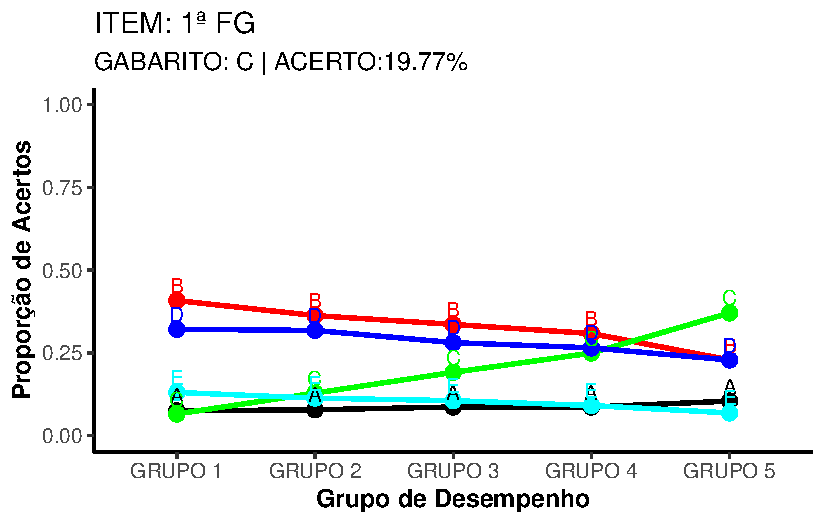
\includegraphics[keepaspectratio]{ANALYSIS_BY_COURSE/SISTEMAS_INFO_files/figure-pdf/fig-PLOT_ITEM_ANALIZER-1.pdf}}

}

\caption{\label{fig-PLOT_ITEM_ANALIZER-1}Análise de um Item Específico
por Grupo de Desempenho discriminando Alternativas da Prova do ENADE
para o Curso de Sitemas de Informação.}

\end{figure}%

\begin{figure}[H]

\centering{

\pandocbounded{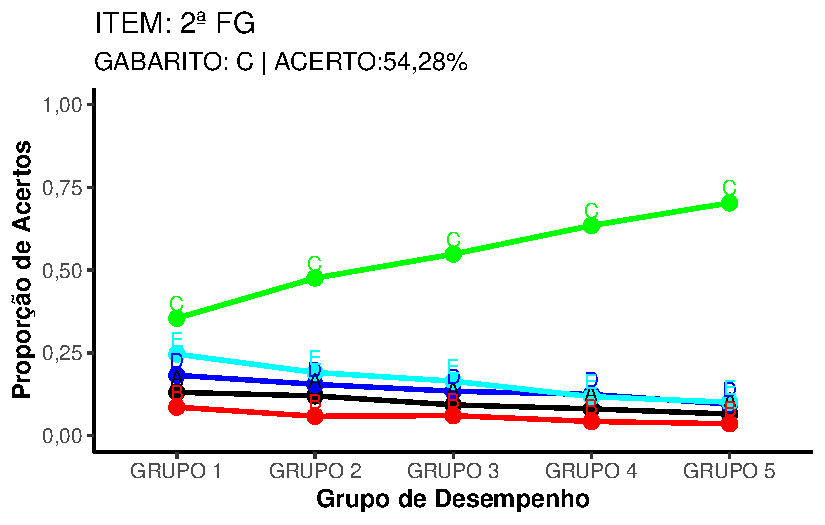
\includegraphics[keepaspectratio]{ANALYSIS_BY_COURSE/SISTEMAS_INFO_files/figure-pdf/fig-PLOT_ITEM_ANALIZER-2.pdf}}

}

\caption{\label{fig-PLOT_ITEM_ANALIZER-2}Análise de um Item Específico
por Grupo de Desempenho discriminando Alternativas da Prova do ENADE
para o Curso de Sitemas de Informação.}

\end{figure}%

\begin{figure}[H]

\centering{

\pandocbounded{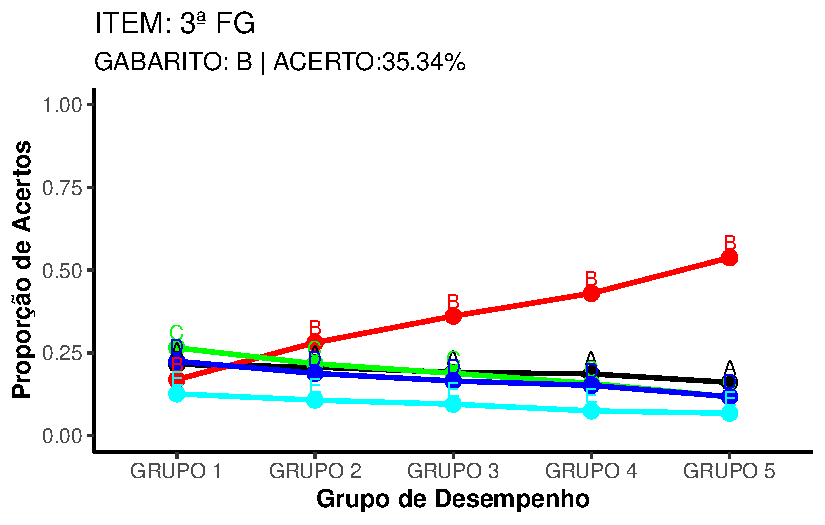
\includegraphics[keepaspectratio]{ANALYSIS_BY_COURSE/SISTEMAS_INFO_files/figure-pdf/fig-PLOT_ITEM_ANALIZER-3.pdf}}

}

\caption{\label{fig-PLOT_ITEM_ANALIZER-3}Análise de um Item Específico
por Grupo de Desempenho discriminando Alternativas da Prova do ENADE
para o Curso de Sitemas de Informação.}

\end{figure}%

\begin{figure}[H]

\centering{

\pandocbounded{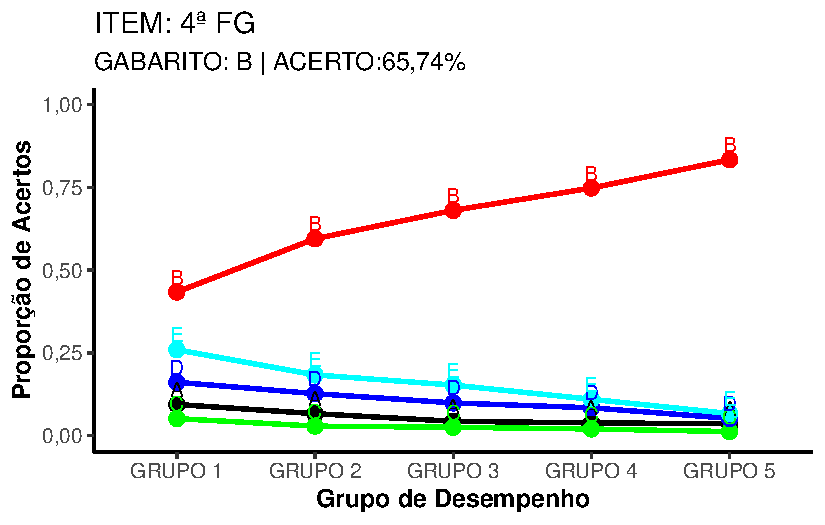
\includegraphics[keepaspectratio]{ANALYSIS_BY_COURSE/SISTEMAS_INFO_files/figure-pdf/fig-PLOT_ITEM_ANALIZER-4.pdf}}

}

\caption{\label{fig-PLOT_ITEM_ANALIZER-4}Análise de um Item Específico
por Grupo de Desempenho discriminando Alternativas da Prova do ENADE
para o Curso de Sitemas de Informação.}

\end{figure}%

\begin{figure}[H]

\centering{

\pandocbounded{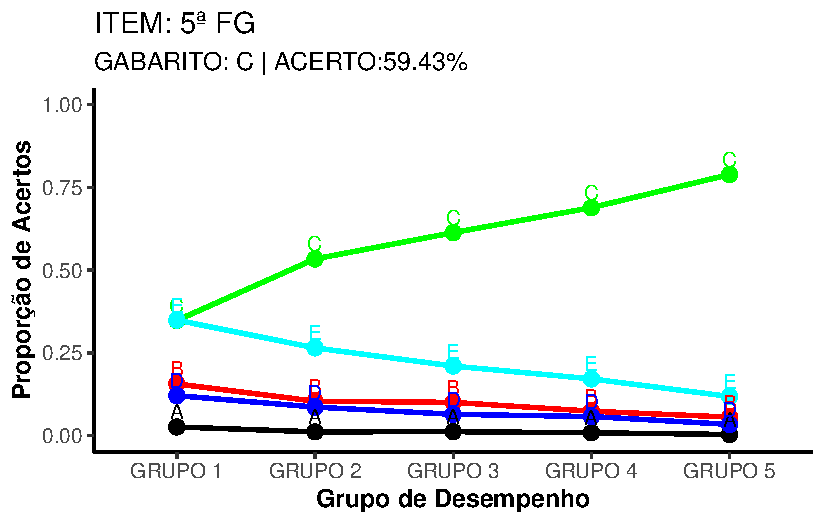
\includegraphics[keepaspectratio]{ANALYSIS_BY_COURSE/SISTEMAS_INFO_files/figure-pdf/fig-PLOT_ITEM_ANALIZER-5.pdf}}

}

\caption{\label{fig-PLOT_ITEM_ANALIZER-5}Análise de um Item Específico
por Grupo de Desempenho discriminando Alternativas da Prova do ENADE
para o Curso de Sitemas de Informação.}

\end{figure}%

\begin{figure}[H]

\centering{

\pandocbounded{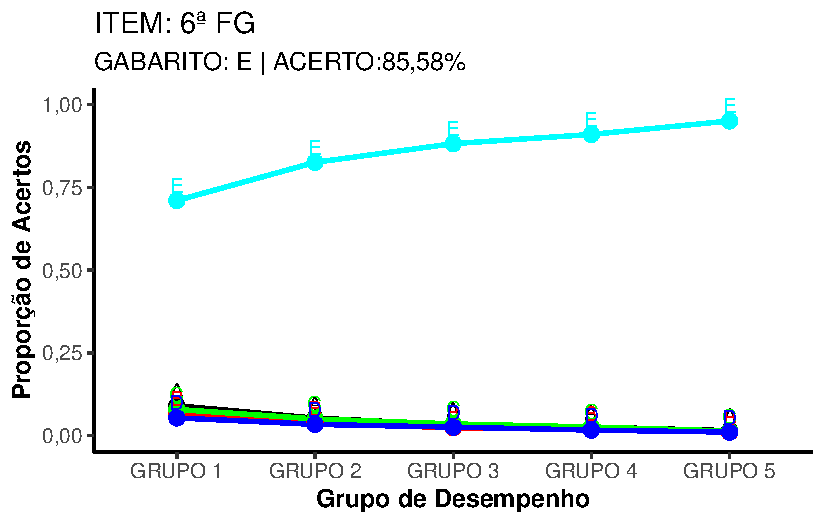
\includegraphics[keepaspectratio]{ANALYSIS_BY_COURSE/SISTEMAS_INFO_files/figure-pdf/fig-PLOT_ITEM_ANALIZER-6.pdf}}

}

\caption{\label{fig-PLOT_ITEM_ANALIZER-6}Análise de um Item Específico
por Grupo de Desempenho discriminando Alternativas da Prova do ENADE
para o Curso de Sitemas de Informação.}

\end{figure}%

\begin{figure}[H]

\centering{

\pandocbounded{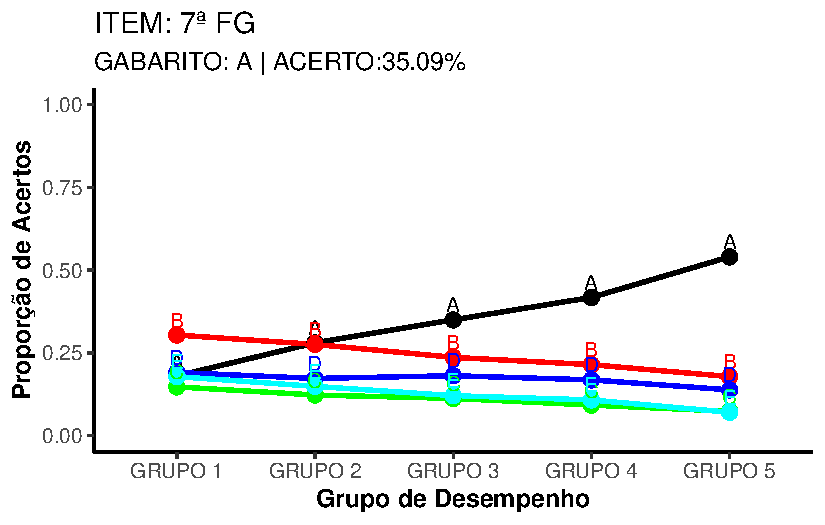
\includegraphics[keepaspectratio]{ANALYSIS_BY_COURSE/SISTEMAS_INFO_files/figure-pdf/fig-PLOT_ITEM_ANALIZER-7.pdf}}

}

\caption{\label{fig-PLOT_ITEM_ANALIZER-7}Análise de um Item Específico
por Grupo de Desempenho discriminando Alternativas da Prova do ENADE
para o Curso de Sitemas de Informação.}

\end{figure}%

\begin{figure}[H]

\centering{

\pandocbounded{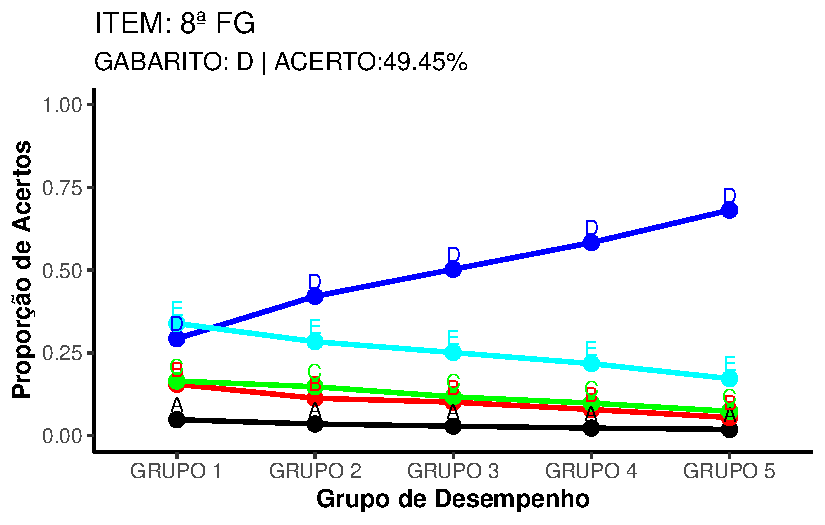
\includegraphics[keepaspectratio]{ANALYSIS_BY_COURSE/SISTEMAS_INFO_files/figure-pdf/fig-PLOT_ITEM_ANALIZER-8.pdf}}

}

\caption{\label{fig-PLOT_ITEM_ANALIZER-8}Análise de um Item Específico
por Grupo de Desempenho discriminando Alternativas da Prova do ENADE
para o Curso de Sitemas de Informação.}

\end{figure}%

\begin{figure}[H]

\centering{

\pandocbounded{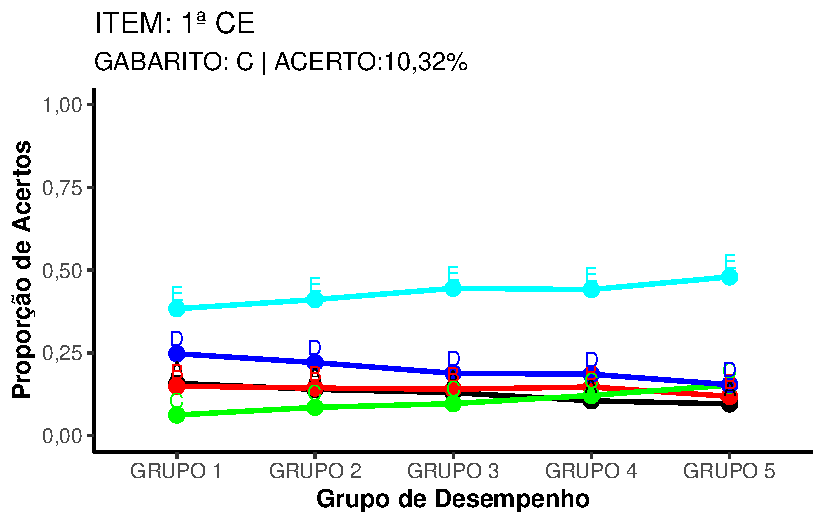
\includegraphics[keepaspectratio]{ANALYSIS_BY_COURSE/SISTEMAS_INFO_files/figure-pdf/fig-PLOT_ITEM_ANALIZER-9.pdf}}

}

\caption{\label{fig-PLOT_ITEM_ANALIZER-9}Análise de um Item Específico
por Grupo de Desempenho discriminando Alternativas da Prova do ENADE
para o Curso de Sitemas de Informação.}

\end{figure}%

\begin{figure}[H]

\centering{

\pandocbounded{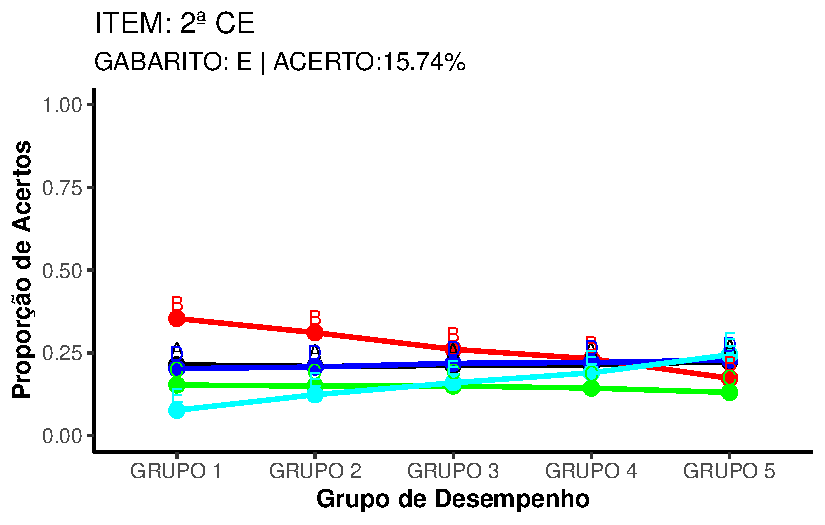
\includegraphics[keepaspectratio]{ANALYSIS_BY_COURSE/SISTEMAS_INFO_files/figure-pdf/fig-PLOT_ITEM_ANALIZER-10.pdf}}

}

\caption{\label{fig-PLOT_ITEM_ANALIZER-10}Análise de um Item Específico
por Grupo de Desempenho discriminando Alternativas da Prova do ENADE
para o Curso de Sitemas de Informação.}

\end{figure}%

\begin{figure}[H]

\centering{

\pandocbounded{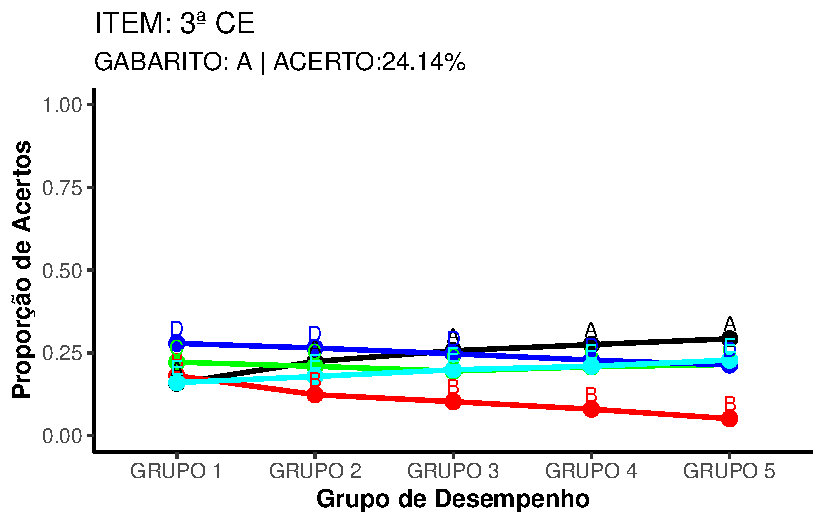
\includegraphics[keepaspectratio]{ANALYSIS_BY_COURSE/SISTEMAS_INFO_files/figure-pdf/fig-PLOT_ITEM_ANALIZER-11.pdf}}

}

\caption{\label{fig-PLOT_ITEM_ANALIZER-11}Análise de um Item Específico
por Grupo de Desempenho discriminando Alternativas da Prova do ENADE
para o Curso de Sitemas de Informação.}

\end{figure}%

\begin{figure}[H]

\centering{

\pandocbounded{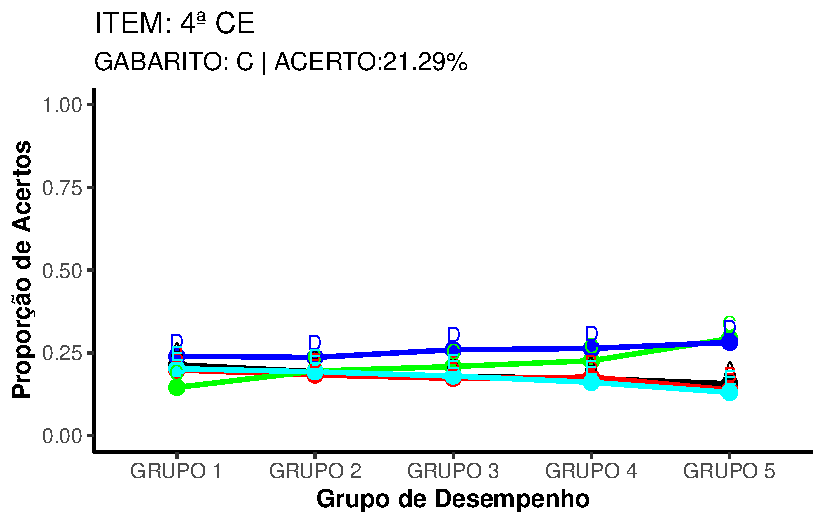
\includegraphics[keepaspectratio]{ANALYSIS_BY_COURSE/SISTEMAS_INFO_files/figure-pdf/fig-PLOT_ITEM_ANALIZER-12.pdf}}

}

\caption{\label{fig-PLOT_ITEM_ANALIZER-12}Análise de um Item Específico
por Grupo de Desempenho discriminando Alternativas da Prova do ENADE
para o Curso de Sitemas de Informação.}

\end{figure}%

\begin{figure}[H]

\centering{

\pandocbounded{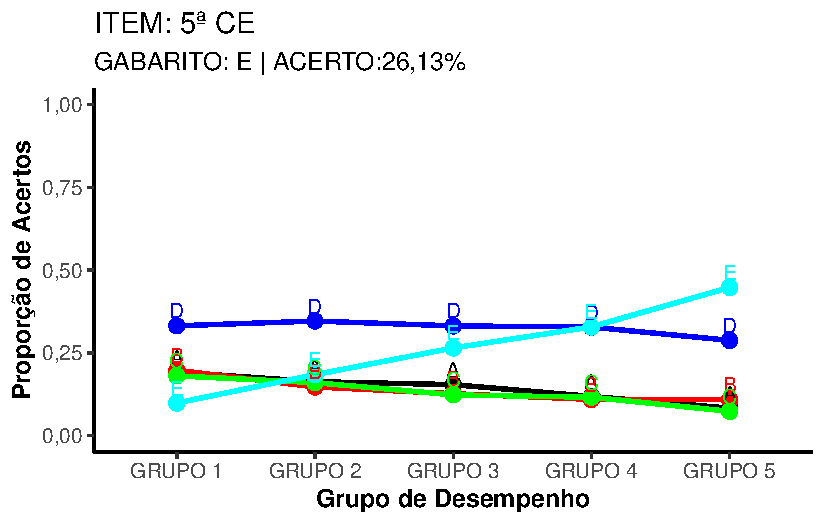
\includegraphics[keepaspectratio]{ANALYSIS_BY_COURSE/SISTEMAS_INFO_files/figure-pdf/fig-PLOT_ITEM_ANALIZER-13.pdf}}

}

\caption{\label{fig-PLOT_ITEM_ANALIZER-13}Análise de um Item Específico
por Grupo de Desempenho discriminando Alternativas da Prova do ENADE
para o Curso de Sitemas de Informação.}

\end{figure}%

\begin{figure}[H]

\centering{

\pandocbounded{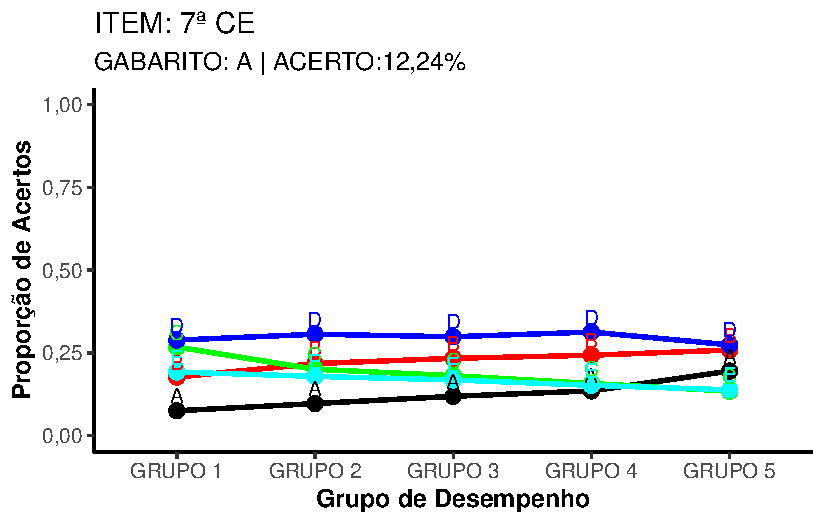
\includegraphics[keepaspectratio]{ANALYSIS_BY_COURSE/SISTEMAS_INFO_files/figure-pdf/fig-PLOT_ITEM_ANALIZER-14.pdf}}

}

\caption{\label{fig-PLOT_ITEM_ANALIZER-14}Análise de um Item Específico
por Grupo de Desempenho discriminando Alternativas da Prova do ENADE
para o Curso de Sitemas de Informação.}

\end{figure}%

\begin{figure}[H]

\centering{

\pandocbounded{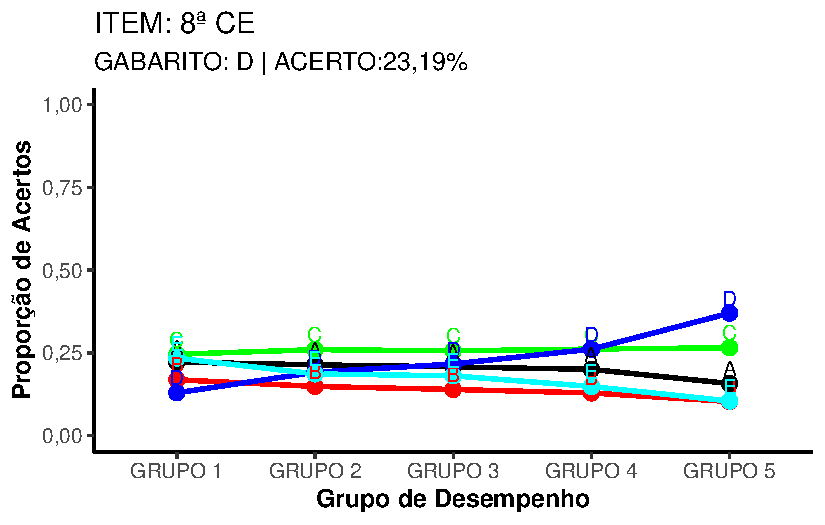
\includegraphics[keepaspectratio]{ANALYSIS_BY_COURSE/SISTEMAS_INFO_files/figure-pdf/fig-PLOT_ITEM_ANALIZER-15.pdf}}

}

\caption{\label{fig-PLOT_ITEM_ANALIZER-15}Análise de um Item Específico
por Grupo de Desempenho discriminando Alternativas da Prova do ENADE
para o Curso de Sitemas de Informação.}

\end{figure}%

\begin{figure}[H]

\centering{

\pandocbounded{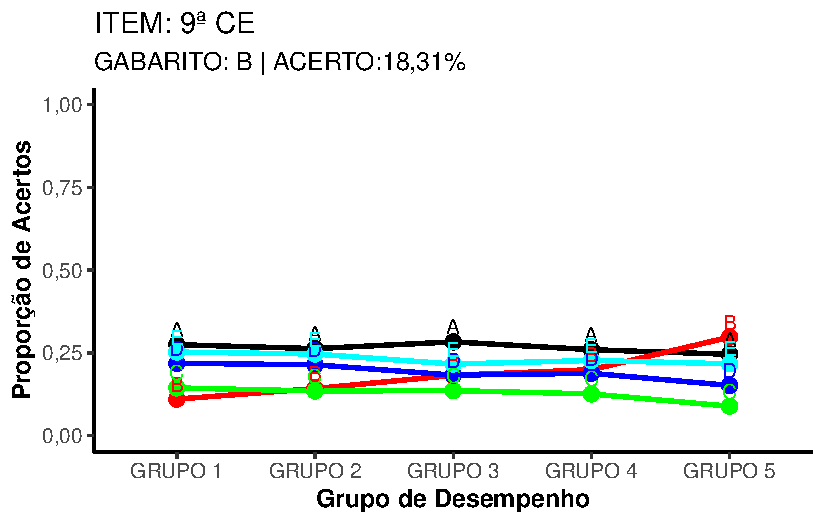
\includegraphics[keepaspectratio]{ANALYSIS_BY_COURSE/SISTEMAS_INFO_files/figure-pdf/fig-PLOT_ITEM_ANALIZER-16.pdf}}

}

\caption{\label{fig-PLOT_ITEM_ANALIZER-16}Análise de um Item Específico
por Grupo de Desempenho discriminando Alternativas da Prova do ENADE
para o Curso de Sitemas de Informação.}

\end{figure}%

\begin{figure}[H]

\centering{

\pandocbounded{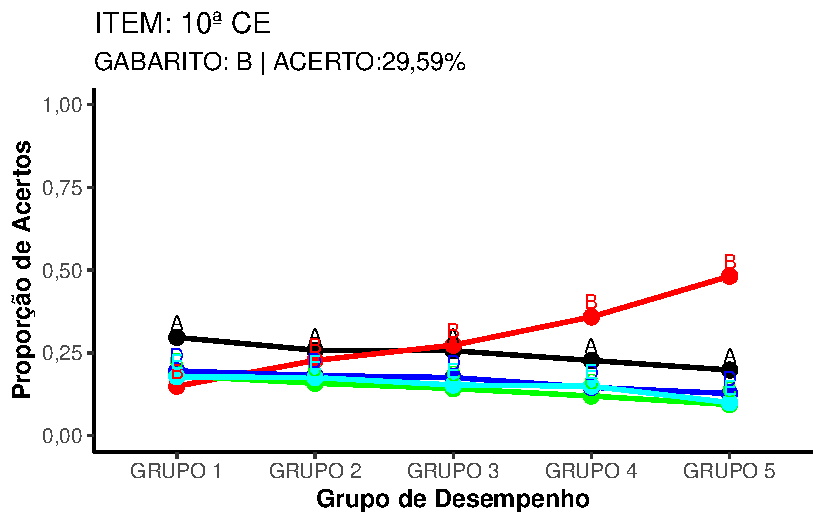
\includegraphics[keepaspectratio]{ANALYSIS_BY_COURSE/SISTEMAS_INFO_files/figure-pdf/fig-PLOT_ITEM_ANALIZER-17.pdf}}

}

\caption{\label{fig-PLOT_ITEM_ANALIZER-17}Análise de um Item Específico
por Grupo de Desempenho discriminando Alternativas da Prova do ENADE
para o Curso de Sitemas de Informação.}

\end{figure}%

\begin{figure}[H]

\centering{

\pandocbounded{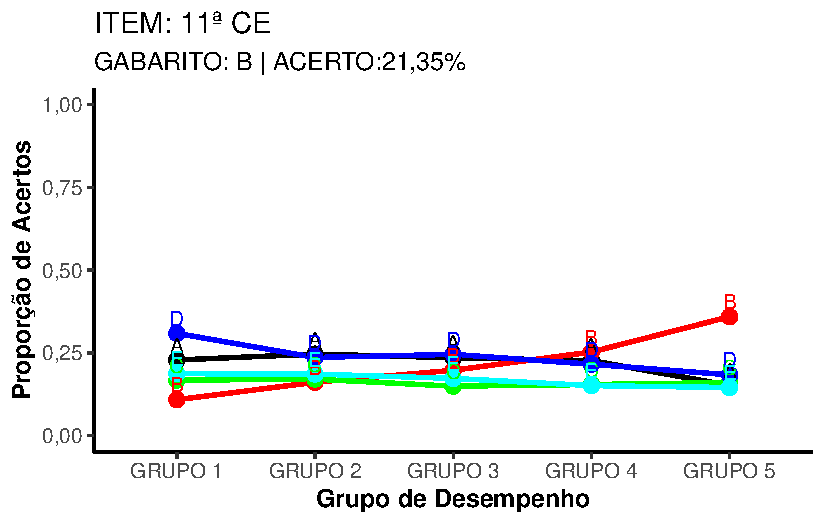
\includegraphics[keepaspectratio]{ANALYSIS_BY_COURSE/SISTEMAS_INFO_files/figure-pdf/fig-PLOT_ITEM_ANALIZER-18.pdf}}

}

\caption{\label{fig-PLOT_ITEM_ANALIZER-18}Análise de um Item Específico
por Grupo de Desempenho discriminando Alternativas da Prova do ENADE
para o Curso de Sitemas de Informação.}

\end{figure}%

\begin{figure}[H]

\centering{

\pandocbounded{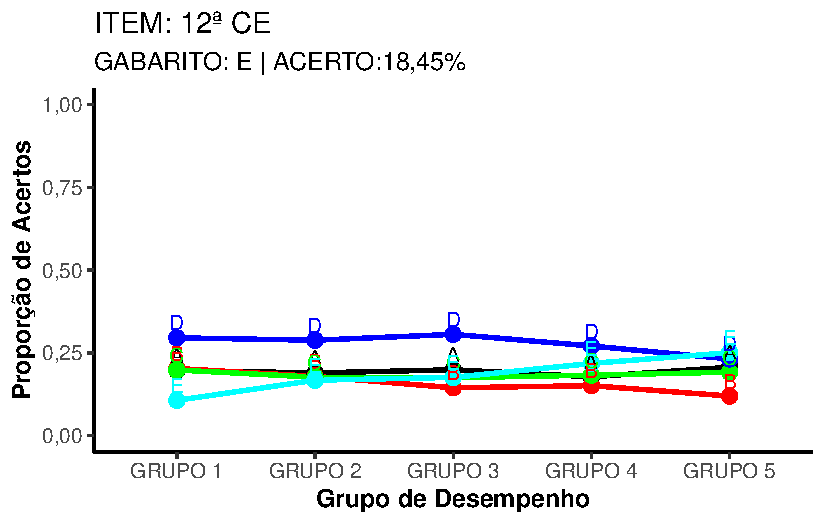
\includegraphics[keepaspectratio]{ANALYSIS_BY_COURSE/SISTEMAS_INFO_files/figure-pdf/fig-PLOT_ITEM_ANALIZER-19.pdf}}

}

\caption{\label{fig-PLOT_ITEM_ANALIZER-19}Análise de um Item Específico
por Grupo de Desempenho discriminando Alternativas da Prova do ENADE
para o Curso de Sitemas de Informação.}

\end{figure}%

\begin{figure}[H]

\centering{

\pandocbounded{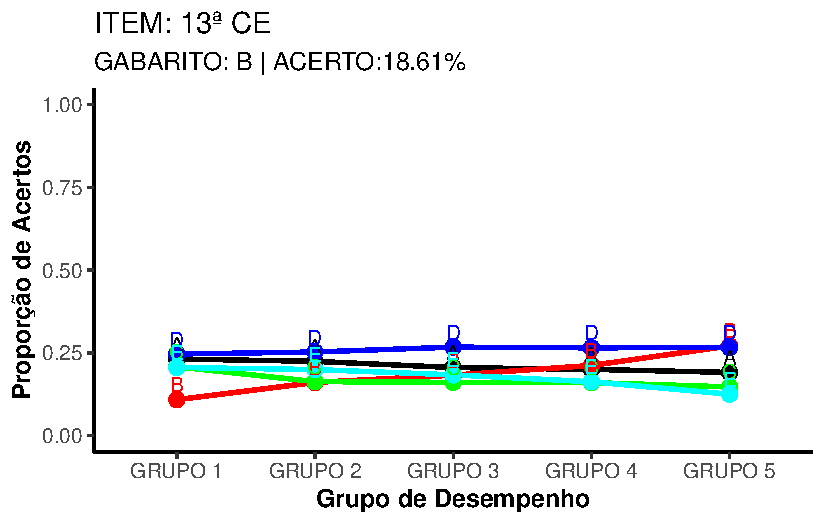
\includegraphics[keepaspectratio]{ANALYSIS_BY_COURSE/SISTEMAS_INFO_files/figure-pdf/fig-PLOT_ITEM_ANALIZER-20.pdf}}

}

\caption{\label{fig-PLOT_ITEM_ANALIZER-20}Análise de um Item Específico
por Grupo de Desempenho discriminando Alternativas da Prova do ENADE
para o Curso de Sitemas de Informação.}

\end{figure}%

\begin{figure}[H]

\centering{

\pandocbounded{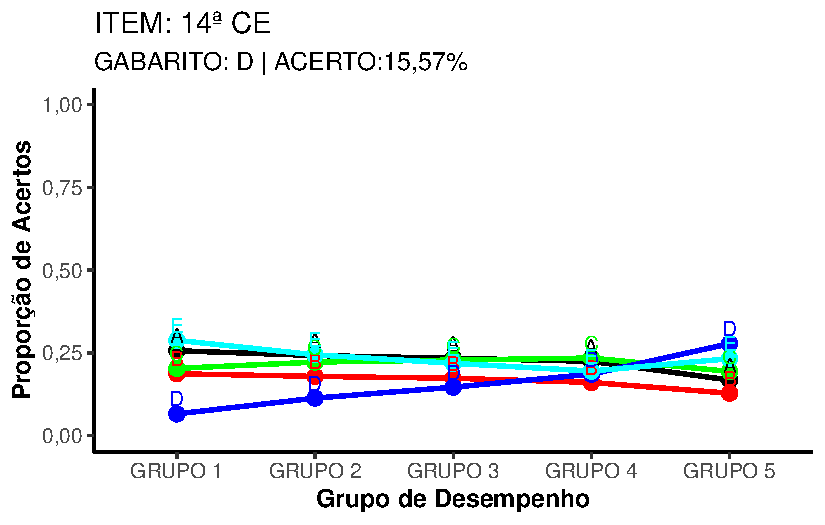
\includegraphics[keepaspectratio]{ANALYSIS_BY_COURSE/SISTEMAS_INFO_files/figure-pdf/fig-PLOT_ITEM_ANALIZER-21.pdf}}

}

\caption{\label{fig-PLOT_ITEM_ANALIZER-21}Análise de um Item Específico
por Grupo de Desempenho discriminando Alternativas da Prova do ENADE
para o Curso de Sitemas de Informação.}

\end{figure}%

\begin{figure}[H]

\centering{

\pandocbounded{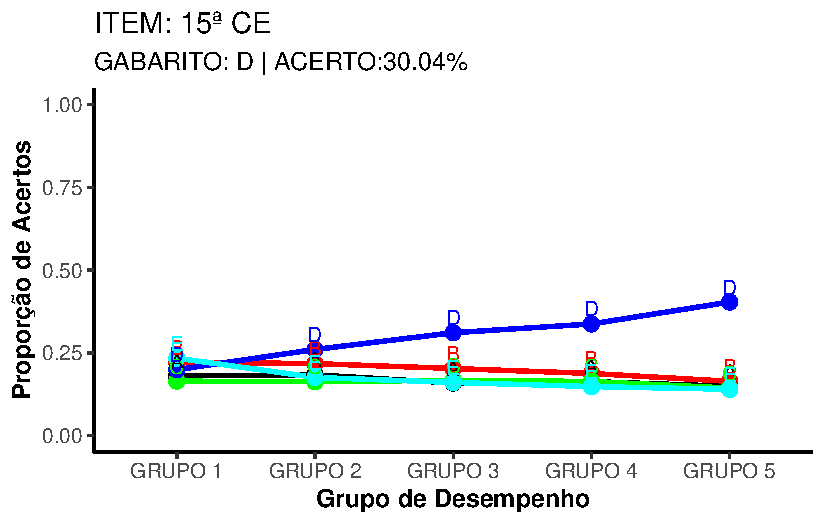
\includegraphics[keepaspectratio]{ANALYSIS_BY_COURSE/SISTEMAS_INFO_files/figure-pdf/fig-PLOT_ITEM_ANALIZER-22.pdf}}

}

\caption{\label{fig-PLOT_ITEM_ANALIZER-22}Análise de um Item Específico
por Grupo de Desempenho discriminando Alternativas da Prova do ENADE
para o Curso de Sitemas de Informação.}

\end{figure}%

\begin{figure}[H]

\centering{

\pandocbounded{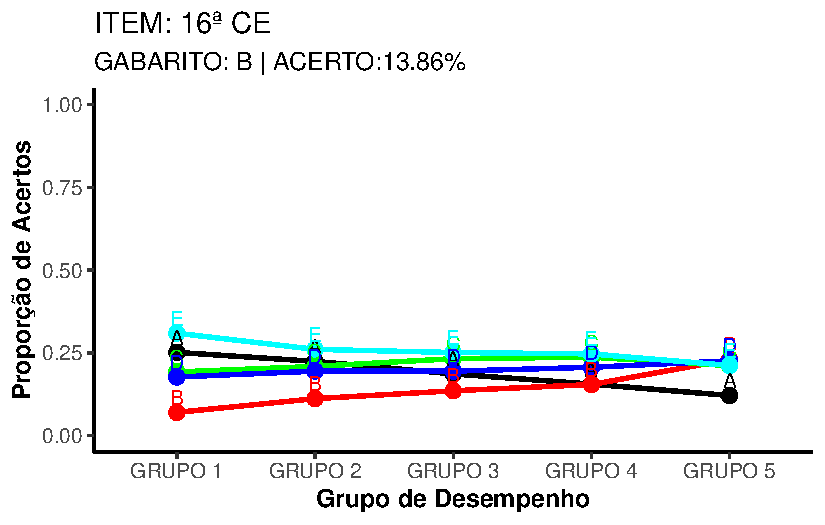
\includegraphics[keepaspectratio]{ANALYSIS_BY_COURSE/SISTEMAS_INFO_files/figure-pdf/fig-PLOT_ITEM_ANALIZER-23.pdf}}

}

\caption{\label{fig-PLOT_ITEM_ANALIZER-23}Análise de um Item Específico
por Grupo de Desempenho discriminando Alternativas da Prova do ENADE
para o Curso de Sitemas de Informação.}

\end{figure}%

\begin{figure}[H]

\centering{

\pandocbounded{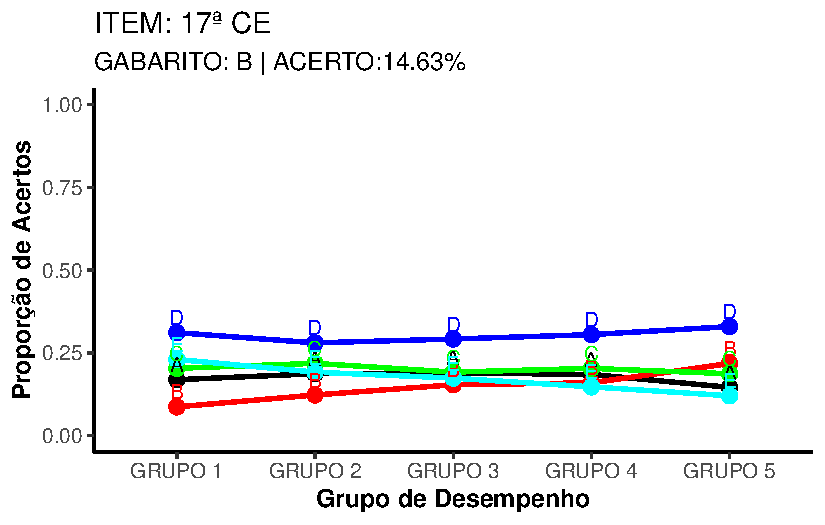
\includegraphics[keepaspectratio]{ANALYSIS_BY_COURSE/SISTEMAS_INFO_files/figure-pdf/fig-PLOT_ITEM_ANALIZER-24.pdf}}

}

\caption{\label{fig-PLOT_ITEM_ANALIZER-24}Análise de um Item Específico
por Grupo de Desempenho discriminando Alternativas da Prova do ENADE
para o Curso de Sitemas de Informação.}

\end{figure}%

\begin{figure}[H]

\centering{

\pandocbounded{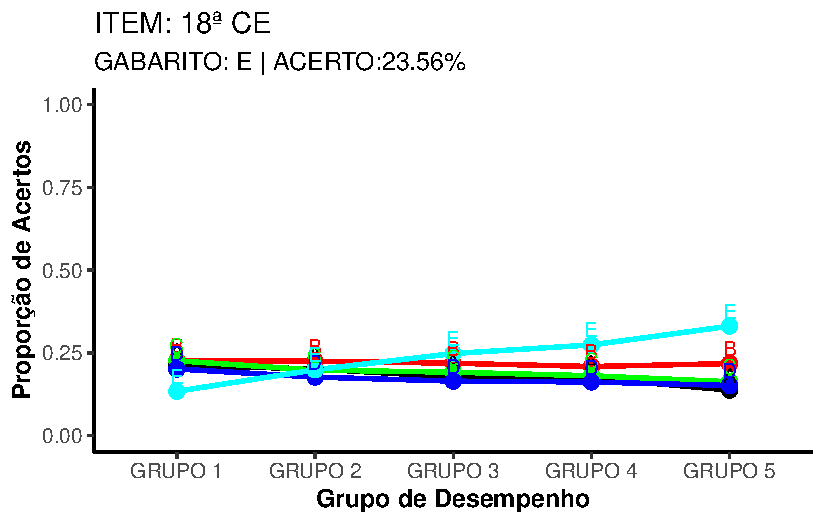
\includegraphics[keepaspectratio]{ANALYSIS_BY_COURSE/SISTEMAS_INFO_files/figure-pdf/fig-PLOT_ITEM_ANALIZER-25.pdf}}

}

\caption{\label{fig-PLOT_ITEM_ANALIZER-25}Análise de um Item Específico
por Grupo de Desempenho discriminando Alternativas da Prova do ENADE
para o Curso de Sitemas de Informação.}

\end{figure}%

\begin{figure}[H]

\centering{

\pandocbounded{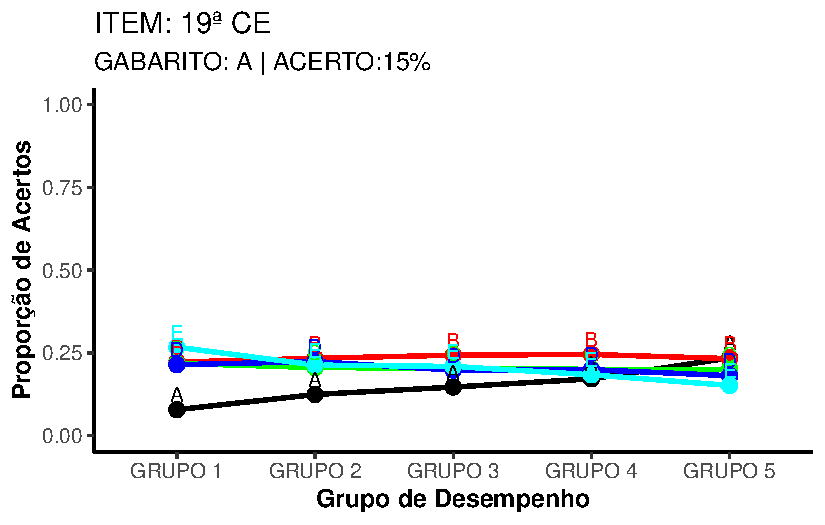
\includegraphics[keepaspectratio]{ANALYSIS_BY_COURSE/SISTEMAS_INFO_files/figure-pdf/fig-PLOT_ITEM_ANALIZER-26.pdf}}

}

\caption{\label{fig-PLOT_ITEM_ANALIZER-26}Análise de um Item Específico
por Grupo de Desempenho discriminando Alternativas da Prova do ENADE
para o Curso de Sitemas de Informação.}

\end{figure}%

\begin{figure}[H]

\centering{

\pandocbounded{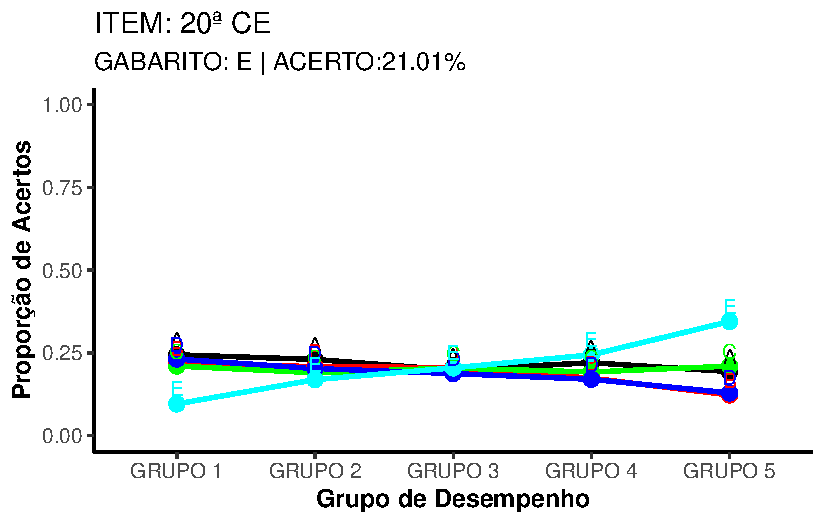
\includegraphics[keepaspectratio]{ANALYSIS_BY_COURSE/SISTEMAS_INFO_files/figure-pdf/fig-PLOT_ITEM_ANALIZER-27.pdf}}

}

\caption{\label{fig-PLOT_ITEM_ANALIZER-27}Análise de um Item Específico
por Grupo de Desempenho discriminando Alternativas da Prova do ENADE
para o Curso de Sitemas de Informação.}

\end{figure}%

\begin{figure}[H]

\centering{

\pandocbounded{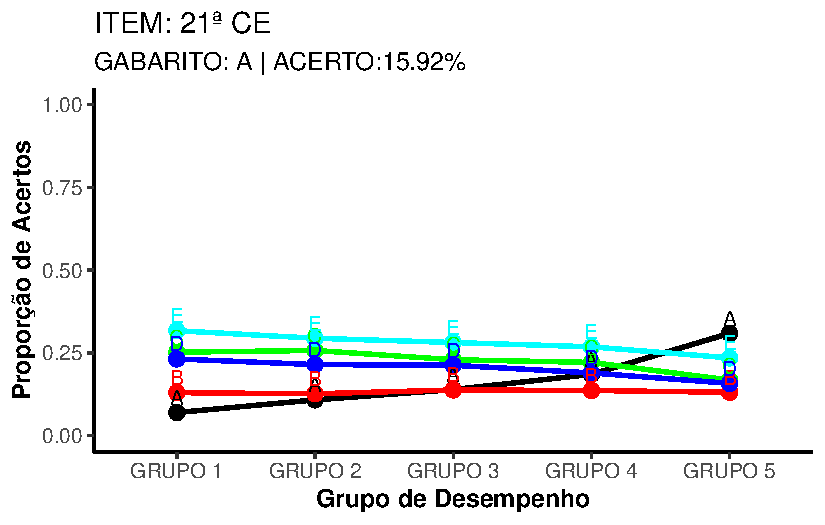
\includegraphics[keepaspectratio]{ANALYSIS_BY_COURSE/SISTEMAS_INFO_files/figure-pdf/fig-PLOT_ITEM_ANALIZER-28.pdf}}

}

\caption{\label{fig-PLOT_ITEM_ANALIZER-28}Análise de um Item Específico
por Grupo de Desempenho discriminando Alternativas da Prova do ENADE
para o Curso de Sitemas de Informação.}

\end{figure}%

\begin{figure}[H]

\centering{

\pandocbounded{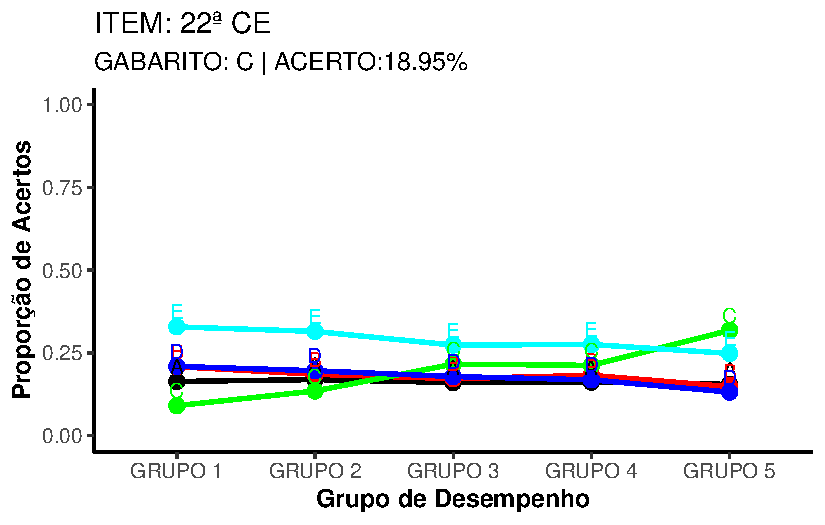
\includegraphics[keepaspectratio]{ANALYSIS_BY_COURSE/SISTEMAS_INFO_files/figure-pdf/fig-PLOT_ITEM_ANALIZER-29.pdf}}

}

\caption{\label{fig-PLOT_ITEM_ANALIZER-29}Análise de um Item Específico
por Grupo de Desempenho discriminando Alternativas da Prova do ENADE
para o Curso de Sitemas de Informação.}

\end{figure}%

\begin{figure}[H]

\centering{

\pandocbounded{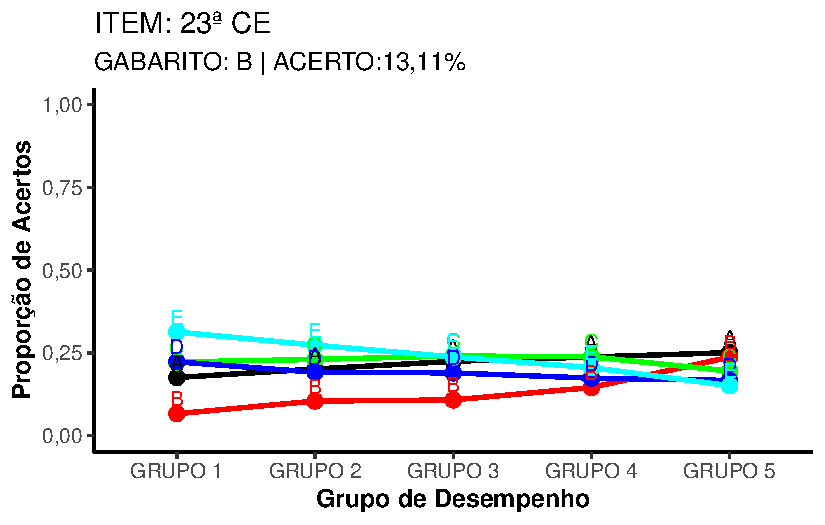
\includegraphics[keepaspectratio]{ANALYSIS_BY_COURSE/SISTEMAS_INFO_files/figure-pdf/fig-PLOT_ITEM_ANALIZER-30.pdf}}

}

\caption{\label{fig-PLOT_ITEM_ANALIZER-30}Análise de um Item Específico
por Grupo de Desempenho discriminando Alternativas da Prova do ENADE
para o Curso de Sitemas de Informação.}

\end{figure}%

\begin{figure}[H]

\centering{

\pandocbounded{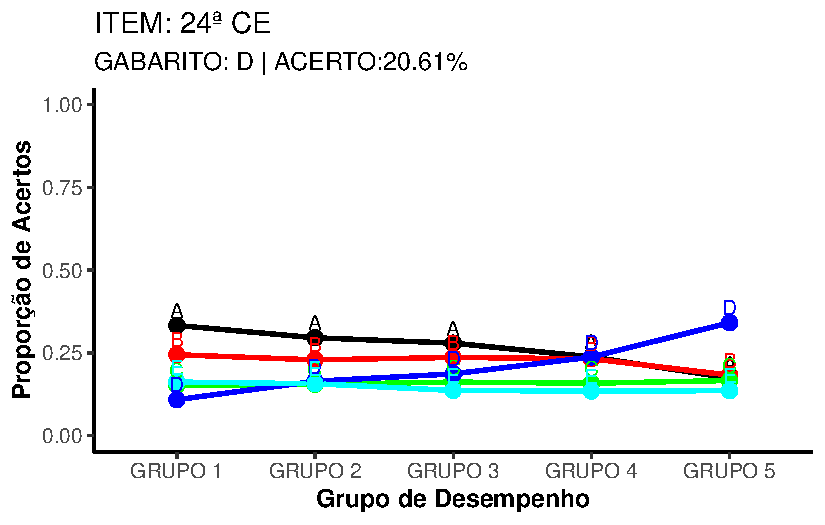
\includegraphics[keepaspectratio]{ANALYSIS_BY_COURSE/SISTEMAS_INFO_files/figure-pdf/fig-PLOT_ITEM_ANALIZER-31.pdf}}

}

\caption{\label{fig-PLOT_ITEM_ANALIZER-31}Análise de um Item Específico
por Grupo de Desempenho discriminando Alternativas da Prova do ENADE
para o Curso de Sitemas de Informação.}

\end{figure}%

\begin{figure}[H]

\centering{

\pandocbounded{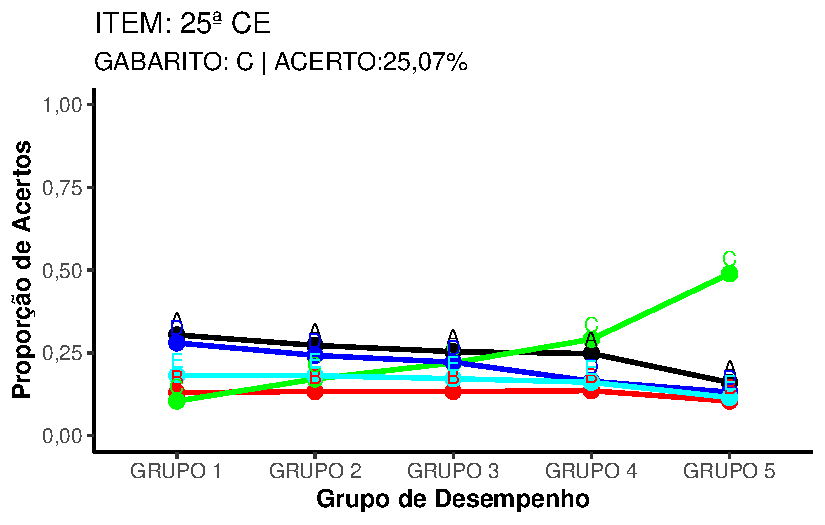
\includegraphics[keepaspectratio]{ANALYSIS_BY_COURSE/SISTEMAS_INFO_files/figure-pdf/fig-PLOT_ITEM_ANALIZER-32.pdf}}

}

\caption{\label{fig-PLOT_ITEM_ANALIZER-32}Análise de um Item Específico
por Grupo de Desempenho discriminando Alternativas da Prova do ENADE
para o Curso de Sitemas de Informação.}

\end{figure}%

\begin{figure}[H]

\centering{

\pandocbounded{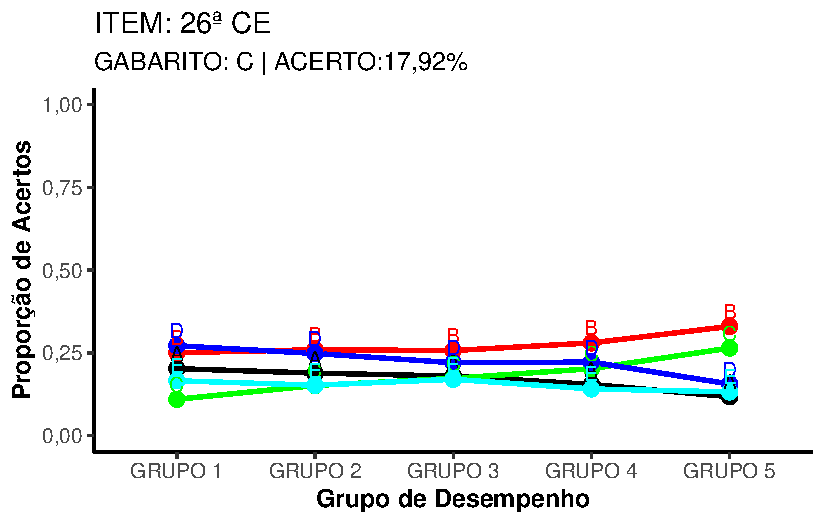
\includegraphics[keepaspectratio]{ANALYSIS_BY_COURSE/SISTEMAS_INFO_files/figure-pdf/fig-PLOT_ITEM_ANALIZER-33.pdf}}

}

\caption{\label{fig-PLOT_ITEM_ANALIZER-33}Análise de um Item Específico
por Grupo de Desempenho discriminando Alternativas da Prova do ENADE
para o Curso de Sitemas de Informação.}

\end{figure}%

\begin{figure}[H]

\centering{

\pandocbounded{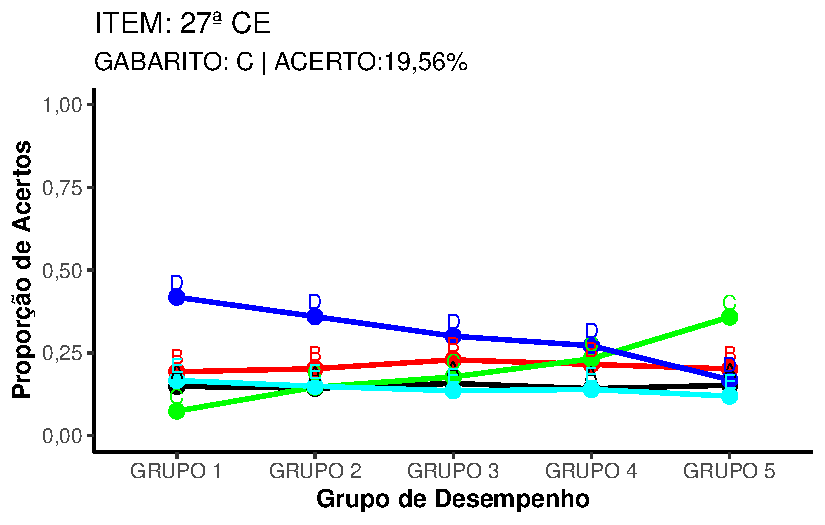
\includegraphics[keepaspectratio]{ANALYSIS_BY_COURSE/SISTEMAS_INFO_files/figure-pdf/fig-PLOT_ITEM_ANALIZER-34.pdf}}

}

\caption{\label{fig-PLOT_ITEM_ANALIZER-34}Análise de um Item Específico
por Grupo de Desempenho discriminando Alternativas da Prova do ENADE
para o Curso de Sitemas de Informação.}

\end{figure}%

\section{Análise via Teoria de Resposta ao Item
(TRI)}\label{anuxe1lise-via-teoria-de-resposta-ao-item-tri}

\bookmarksetup{startatroot}

\chapter*{Referências}\label{referuxeancias}
\addcontentsline{toc}{chapter}{Referências}

\markboth{Referências}{Referências}

\phantomsection\label{refs}




\end{document}
